\documentclass[a4paper, 12pt]{article}
\usepackage[hmargin=1.25in,vmargin=1in]{geometry}

\usepackage{xeCJK}

%% Font
\CJKfontspec{Noto Serif CJK TC} % 思源宋體

\usepackage{parskip}
\setlength{\parindent}{2em} % 縮排兩個字
\usepackage{indentfirst}
\usepackage{makecell}
\usepackage{listings} % Maybe for code block
\usepackage{underscore}

% If you don't like separate files, use this:
% \usepackage{filecontents}
% \begin{filecontents}{references.bib}
% @online{csie_restaurant,
%   author = "{guyleaf, asd3013593, RonToSucceed, a58176197, Andersonabc, orz123789}",
%   title = "CSIE restaurant 孜宮庭園-北科大校園外送平台",
%   url  = "https://github.com/guyleaf/csie_restaurant",
% }
% @online{aws_arch_diagram,
%   author = "Amazon Web Services",
%   title = "What Is Architecture Diagramming?",
%   url  = "https://aws.amazon.com/what-is/architecture-diagramming",
% }
% \end{filecontents}

\usepackage[autocite=superscript]{biblatex}
\addbibresource{references.bib}

\usepackage{graphicx}
\graphicspath{ {./images/} }

\usepackage{hyperref}
\hypersetup{
    colorlinks=true,
    linkcolor=black,
    filecolor=magenta,      
    urlcolor=cyan,
    pdftitle={Overleaf Example},
    pdfpagemode=FullScreen,
} % Copy from https://www.overleaf.com/learn/latex/Hyperlinks

% Custom varibles
\def\myProjectName{PUN street Universal Access (PUA)}
\def\myVersion{1.0}

% Font Size
\newcommand\TwentyTitle{\fontsize{20pt}{24pt}\selectfont}
\newcommand\EighteenTitle{\fontsize{18pt}{20pt}\selectfont}
\newcommand\SixteenTitle{\fontsize{16pt}{18pt}\selectfont}
\newcommand\SectionFont{\fontsize{14pt}{16pt}\selectfont}
\newcommand\NormalFont{\fontsize{12pt}{16pt}\selectfont}

\usepackage{titlesec}
\titleformat*{\section}{\center\SectionFont\bfseries}
\titleformat*{\subsection}{\NormalFont\bfseries}
\titleformat*{\subsubsection}{\NormalFont}

\renewcommand{\arraystretch}{1.2} % table row height

%----------------------------------------------------------

\begin{document}

\definecolor{dkgreen}{rgb}{0,0.6,0}
\definecolor{gray}{rgb}{0.5,0.5,0.5}
\definecolor{mauve}{rgb}{0.58,0,0.82}
\definecolor{pink}{rgb}{1,0.41,0.7}

\lstset{
  frame=trbl,
  frameround = tttt,
  language=sql,
  aboveskip=3mm,
  belowskip=3mm,
  showstringspaces=false,
  columns=flexible,
  basicstyle={\small\ttfamily},
  numbers=none,
  numberstyle=\tiny\color{pink},
  keywordstyle=\color{blue},
  commentstyle=\color{dkgreen},
  stringstyle=\color{mauve},
  breaklines=true,
  breakatwhitespace=true,
  tabsize=3,
  morekeywords={REFERENCES, SERIAL, IF},
}


%titlepage
\thispagestyle{empty}
\begin{center}
    {\TwentyTitle \myProjectName \par}
    \vspace{6cm}
    {\TwentyTitle 系統需求規格書 \par}
    {\EighteenTitle Software Requirements Specification (SRS) \par}
    {\SixteenTitle Version: \myVersion \par}
    \vspace{4cm}
    {\SixteenTitle
    \begin{tabular}{ccc}
      姓名 & 學號 & E-mail \\[0.2em]
      郭丞軒 & 110590001 & t110590001@ntut.org.tw \\
      王熯竑 & 110590002 & t110590002@ntut.org.tw \\
      陸艿寰 & 110590007 & t110590007@ntut.org.tw \\
      陳姿安 & 110590017 & t1105900017@ntut.org.tw \\
      劉承翰 & 110590018 & t110590018@ntut.org.tw \\
      歐佳昀 & 110590450 & t110590450@ntut.org.tw \\
    \end{tabular}
    \par}
    \vspace{2cm}
    {\SixteenTitle Department of Computer Science \& Information Engineering National Taipei University of Technology \par}
    \vspace{16pt}
    {\SixteenTitle 10/11/2023 \par}
\end{center}
\clearpage

\renewcommand{\contentsname}{目錄 (Table of Contents)}
\tableofcontents
\newpage

%---------------------------------------------

% \section*{Revision History}

% \begin{center}
%     \begin{tabular}{|c|c|c|c|}
%         \hline
% 	    Name & Date & Reason For Changes & Version\\
%         \hline
% 	    21 & 22 & 23 & 24\\
%         \hline
% 	    31 & 32 & 33 & 34\\
%         \hline
%     \end{tabular}
% \end{center}

% \newpage
%----------------------------------------------


% huhuhu
\section{簡介 (Introduction)}

\subsection{目的 (Purpose)}

光華商場旁的美食街道,俗稱「潘(p'un)街」,是北科學生平日不可或缺的食物來源。每到用餐時段,街道上總是充滿著排隊人潮。為了讓學生們能夠更方便的取得潘街的食物,我們將藉由在資料庫系統課程及過往程式語言及網路通訊的基礎知識,分工合作開發一個美食訂購及外送系統--「PUN street Universal Access」,簡稱PUA。此系統可以讓使用者在網頁上瀏覽、搜尋、並訂購餐點,讓所有人都能夠方便、迅速的享用潘街上的美食。

\noindent 本系統主要目標為:
\begin{enumerate}
  \item 顧客可以瀏覽、搜索店家並訂購餐點
  \item 顧客可以查詢購物車、訂單狀況
  \item 顧客可以為商店評分
  \item 顧客可以註冊商店成為商店管理者
  \item 商店管理者可以管理、更新餐點品項
  \item 商店管理者可以計算月份總銷量、餐點銷售統計資料
  \item 商店管理者可以更新訂單狀況
  \item 商店管理者可以更新、查詢和刪除各種折扣政策
\end{enumerate}


\subsection{系統名稱 (Identification)}

\noindent 本專案範圍包含建置下面主系統與各項子系統,主系統為:

\begin{itemize}
  \item 線上訂餐系統(Web-based Ordering system, WOS)
\end{itemize}

\noindent 子系統為:

\begin{itemize}

% admin
  \item 帳號管理子系統(Account Management Subsystem,AMS)
% staff
  \item 商店註冊子系統(Shop Register Subsystem, SRS)
  \item 商品管理子系統(Commodity Management Subsystem, CMS)
  \item 折扣管理子系統(Discount Management Subsystem, DMS)
  \item 訂單配送管理子系統(Order and Logistics Management Subsystem, OLMS)
  \item 銷售分析子系統(Sales Analysis System, SAS)
% customer
  \item 購物車子系統(Shopping Cart Management Subsystem, SCMS)
  \item 商店評價管理子系統(Comment and Score Management Subsystem, CSMS)
  \item 商品搜尋推薦管理子系統(Search and Recommend Management Subsystem,
SRMS)
  \item 歷史訂單子系統(Historical Order Subsystem, HOS)

% other
  \item 資料庫子系統(Database Subsystem, DBS)

\end{itemize}


\subsection{概觀 (Overview)}

本系統採用前後端分離架構開發,以便團隊成員分工。我們採用svelte作為前端框架,後端利用golang撰寫,資料庫管理系統則使用postgreSQL。


\subsection{符號描述 (Notation Description) (if any)}

\newcommand{\notationDescTableCol}{ | p{6.5em} | p{32em} |}

\noindent \begin{tabular}{ | p{6.5em} | p{32em} |}
  \hline
  Notation & Description \\
  \hline
  WOS 1.0.0 & The WOS components will be labeled with the number 1.0.0 \\
  AMS 1.1.n & The AMS components will be labeled with the number 1.1.n \\
  SRS 1.2.1.n & The SRS components will be labeled with the number 1.2.n \\
  CMS 1.3.n & The CMS components will be labeled with the number 1.3.n \\
  DMS 1.4.n & The DMS components will be labeled with the number 1.4.n \\
  OLMS 1.5.n & The OLMS components will be labeled with the number 1.5.n \\
  SAS 1.6.n & The SAS components will be labeled with the number 1.6.n \\
  SCMS 1.7.n & The SCMS components will be labeled with the number 1.7.n \\
  CSMS 1.8.n & The CSMS components will be labeled with the number 1.8.n \\
  SRMS 1.9.n & The SRMS components will be labeled with the number 1.9.n \\
  HOS 1.10.n & The HOS components will be labeled with the number 1.10.n \\
  DBS 1.11.n & The DBS components will be labeled with the number 1.11.n \\
  \hline
\end{tabular} \par

\noindent \begin{tabular}{ | p{6.5em} | p{32em} |}
  \hline
  Notation & Description \\
  \hline
  WOS-I-nnn & WOS 介面需求(Interface Requirements) \\
  WOS-F-nnn & WOS 功能性需求(Functional Requirements) \\
  WOS-D-nnn & WOS 資料需求(Data Requirements) \\
  WOS-N-nnn & WOS 非功能性需求(Non-Functional Requirements) \\
  WOS-O-nnn & WOS 其他需求(Other Requirements) \\
  WOS-B-nnn & WOS 商業規則或約束 (Business Rules or Constraints) \\
  \hline
\end{tabular} \par

\newpage

\section{系統 (System)}
% huhuhu
\subsection{系統描述 (System Description)}
\subsubsection{系統架構圖 (System Architecture Diagram) }
%\includegraphics[width=30em]{arch-digram.png}

\begin{figure*}[h]
    \centering
    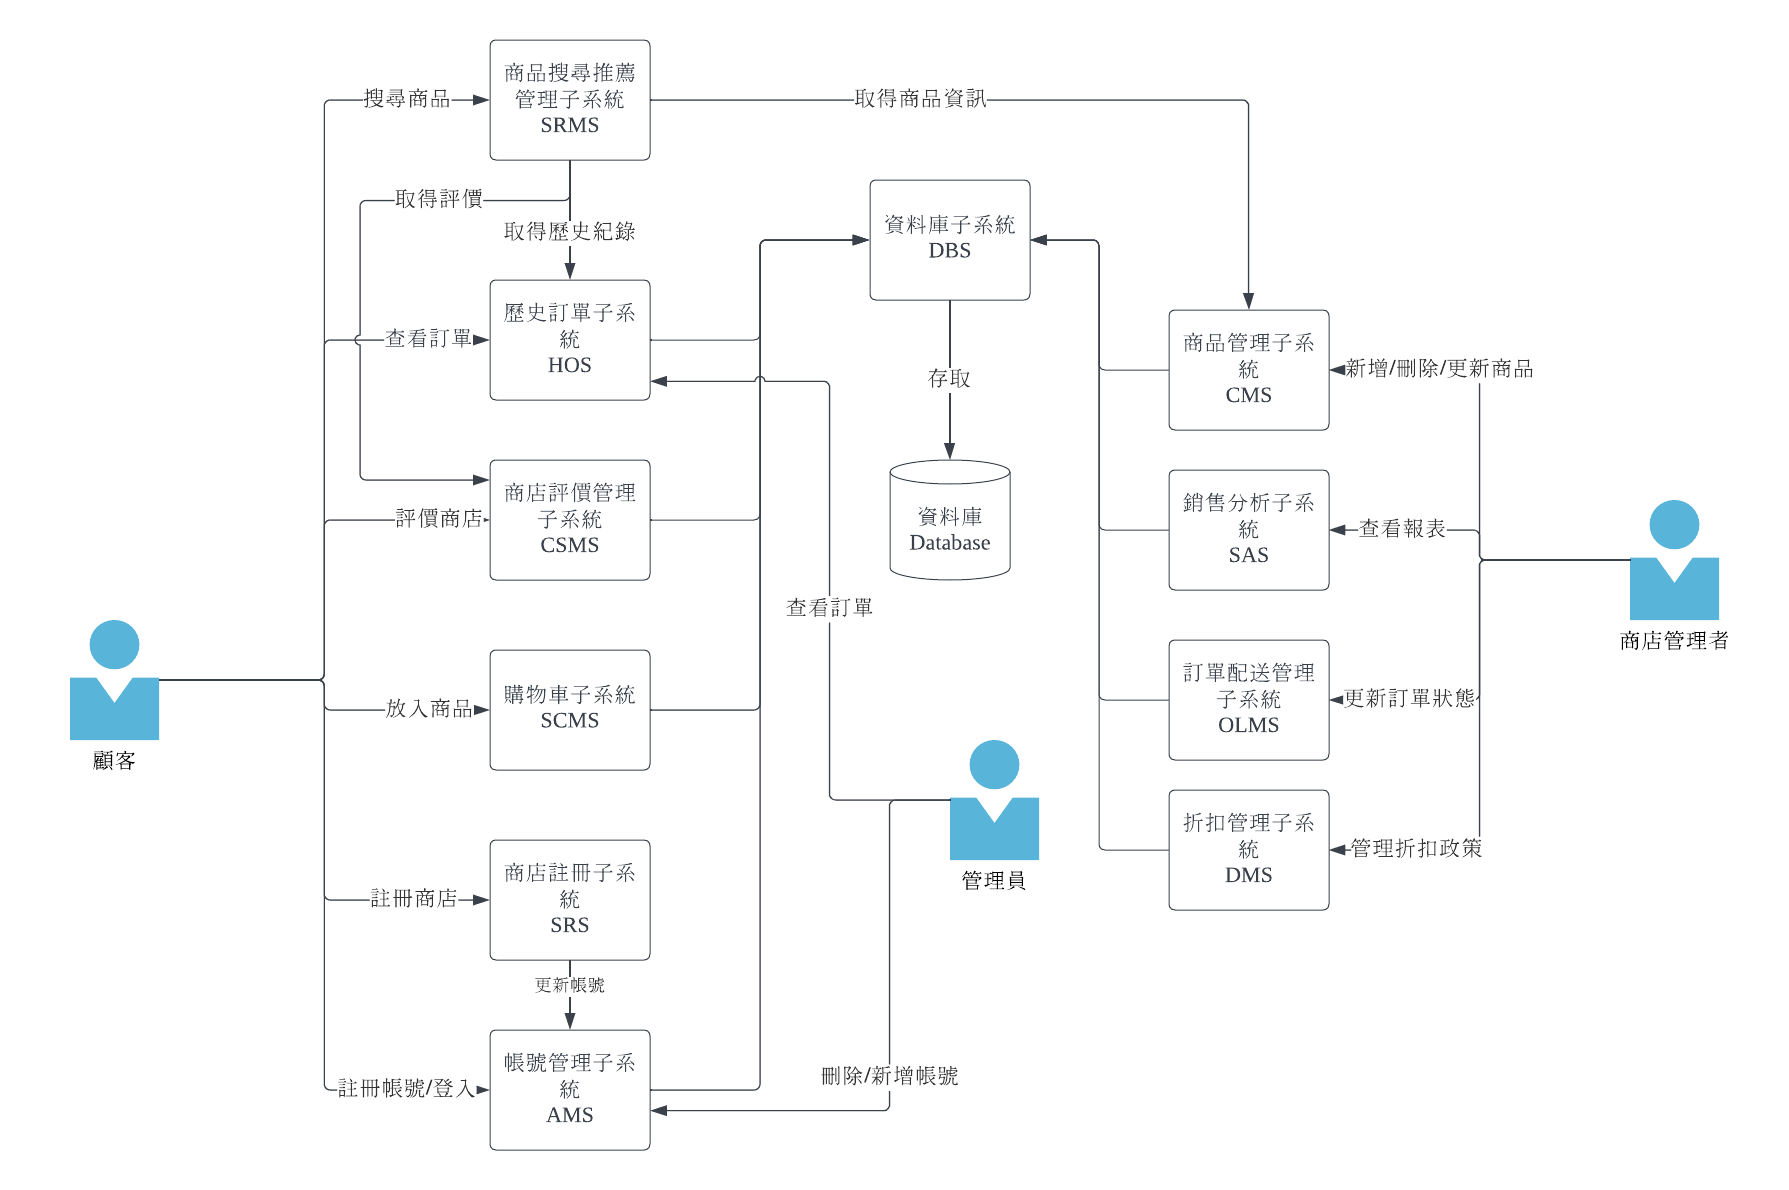
\includegraphics[width=40em]{System-Architecture-Diagram.png}
    \caption{系統架構圖}
    \label{fig:enter-label}
\end{figure*}

%\cite{aws_arch_diagram}

\subsection{操作概念 (Operational Concepts or User Stories)}
\begin{itemize}
 
\item 顧客操作概念: \\
\setlength{\parindent}{2em} 使用者可以透過帳號管理子系統(AMS)進行註冊,用商品搜尋推薦管理子系統(SRMS)尋找自己想要的商品,透過歷史訂單子系統(HOS)查詢自己的訂單歷史紀錄,並透過購物車子系統(SCMS)將商品放入購物車並購買商品。
\item 商店管理者操作概念: \\
\setlength{\parindent}{2em} 顧客可以透過商店註冊系統(SRS)進行註冊成為商店管理者,用商品管理子系統(CMS)管理商品,用銷售分析子系統(SAS)產生財務報表,並透過訂單配送管理子系統(OLMS)管理顧客訂單。
\item 管理員操作概念: \\
\setlength{\parindent}{2em} 管理員可以透過帳號管理子系統(AMS)管理所有帳號,透過歷史訂單子系統(HOS)查看所有訂單紀錄。

\end{itemize}

% glu
\subsection{功能性需求 (Functional Requirements)}

\noindent \begin{tabular}{ | p{6.5em} | p{32em} |}
  \hline
  Notation & Description \\
  \hline
  WOS-F-001 & 顧客可以註冊帳號。 \\
  \hline
  WOS-F-002 & 顧客可以搜尋商店及商品。 \\
  \hline
  WOS-F-003 & 顧客可以將商品加入購物車。 \\
  \hline
  WOS-F-004 & 顧客可以結帳購物車內的商品。 \\
  \hline
  WOS-F-005 & 顧客可以查詢訂單狀態。 \\
  \hline
  WOS-F-006 & 顧客可以在訂單完成後為商店或商品評分。 \\
  \hline
  WOS-F-007 & 顧客可以查詢訂購歷史。 \\
  \hline
  WOS-F-008 & 顧客可以註冊商店成為商店管理員。 \\
  \hline
  WOS-F-009 & 商店管理者可以增加、刪減商品品項及數量。 \\
  \hline
  WOS-F-010 & 商店管理者可以查詢日、周、月銷售量及金額。 \\
  \hline
  WOS-F-011 & 商店管理者可以更新訂單狀況。 \\
  \hline
  WOS-F-012 & 商店管理者可以查詢、增加及刪減各項折扣方案。 \\
  \hline
  WOS-F-013 & 管理員可以新增、刪除、更新帳號。 \\
  \hline
  WOS-F-014 & 管理員可以查看所有訂單。 \\
  \hline
\end{tabular} \par

% lethe
\subsection{資料需求 (Data Requirements)}
\noindent\begin{tabular}{|l| p{32em}|}
    \hline
    需求編號 & 需求描述 \\
    \hline
    WOS-D-001 & 系統需儲存使用者的相關資訊:登入ID、姓名、密碼、電子郵件、地址 \\
    \hline
    WOS-D-002 & 系統需儲存產品的相關資訊:產品ID、名稱描述、其他屬性、產品圖片、價格、庫存產品數量、標籤 \\
    \hline
    WOS-D-003 & 系統需儲存商店的相關資訊:商店ID、名稱、地址、聯絡電子郵件、電話 \\
    \hline
    WOS-D-004 & 系統需儲存訂單的相關資訊:訂單ID、時間、客戶、每個採購項目的名稱和價格、每個採購項目的數量、採購總額、訂單的當前狀態(已接收、處理、運輸、關閉) \\
    \hline
    WOS-D-005 & 系統需儲存銷售報告的相關資訊:日期、商店名稱、訂單數量、銷售總額 \\
    \hline
\end{tabular}

% glu
\subsection{非功能性需求 (Non-Functional Requirements)}
\subsubsection{效能需求 (Performance Requirements)}
\noindent\begin{tabular}{|l| p{32em}|}
    \hline
    需求編號 & 需求描述 \\
    \hline
    WOS-N-001 & 網頁載入時間需不超過五秒 \\
    \hline
    WOS-N-002 & 用戶搜尋時間需不超過五秒 \\
    \hline
    WOS-N-003 & 商店管理員更新訂單及商店狀況至用戶端反映需不超過三十秒 \\
    \hline
\end{tabular}
\subsubsection{資安需求 (Security Requirements)}
\noindent\begin{tabular}{ | p{6.5em} | p{32em} |}
    \hline
    需求編號 & 需求描述 \\
    \hline
    WOS-N-004 & 註冊密碼必須符合複雜度需求 \\
    \hline
    WOS-N-005 & 管理員應遵守隱私權保護政策,不可隨意檢視個人資料 \\
    \hline
\end{tabular}
\subsection{介面需求 (Interface Requirements)}
% orange
\subsubsection{使用者介面需求 (User Interfaces Requirements)}
\setlength{\parindent}{2em} 買家介面
\begin{center}
\noindent\begin{tabular}{ | p{6.5em} | p{32em} |}
    \hline
    需求編號 & 需求描述 \\ 
    \hline
    WOS-I-001 & 搜尋食物or店家種類介面。\\
    \hline
    WOS-I-002 & 購物清單介面\\
    \hline
    WOS-I-003 & 點餐介面。\\
    \hline
    WOS-I-004 & 訂單配送管理界面。\\
    \hline
    \end{tabular}
\end{center}

\setlength{\parindent}{2em} 商家介面
\begin{center}
\noindent\begin{tabular}{ | p{6.5em} | p{32em} |}
    \hline
    需求編號 & 需求描述 \\ 
    \hline
    WOS-I-005 & 刊登商品資訊。\\
    \hline
    WOS-I-006 & 檢視買家訂單\\
    \hline
    WOS-I-007 & 管理刊登商品介面。\\
    \hline
    WOS-I-008 & 折扣管理介面。\\
    \hline
    WOS-I-009 & 檢視銷售報表介面。\\
    \hline
    \end{tabular}
\end{center}
    
\subsubsection{內部介面需求 (Internal Interface Requirements)}
\begin{center}
    \begin{tabular}{ | p{6.5em} | p{32em} |}
    \hline
    需求編號 & 需求描述 \\ 
    \hline
    WOS-I-010 & SRMS能向CMS接收商品資訊需求。\\
    \hline
    WOS-I-011 & SRMS能向HOS接收歷史訂單需求。\\
    \hline
    WOS-I-012 & SRMS能向CSMS接收評價需求。\\
    \hline
    WOS-I-013 & HOS與DBS需有傳送與接收歷史訂單需求。\\
    \hline
    WOS-I-014 & CSMS與DBS需有傳送與接收商店評價需求。\\
    \hline
    WOS-I-015 & SCMS與DBS需有傳送與接收購物車相關資訊需求。\\
    \hline
    WOS-I-016 & SRS能向AMS傳送更新帳號的需求。\\
    \hline
    WOS-I-017 & AMS與DBS需有傳送與接收帳號資訊需求。\\
    \hline
    WOS-I-018 & CMS與DBS需有傳送與接收商品資訊的需求。\\
    \hline
    WOS-I-019 & SAS能向DBS傳送取得銷售分析需求。\\
    \hline
    WOS-I-020 & OLMS能向DBS傳送更新訂單需求。\\
    \hline
    WOS-I-021 & DMS與DBS需有傳送與接收優惠資訊需求。\\
    \hline
    \end{tabular}
\end{center}
% wj4wj4
\subsection{其他需求 (Other Requirements)}
\subsubsection{環境需求 (Environmental Requirement)}
\begin{center}
    \begin{tabular}{ | p{6.5em} | p{32em} |}
    \hline
    需求編號 & 需求說明 \\ 
    \hline
    WOS-O-001 & 需要網路\\ 
    \hline
    WOS-O-002 & docker\\ 
    \hline
    WOS-O-003 & 中子\\ 
    \hline
    WOS-O-004 & 電子\\ 
    \hline
    WOS-O-005 & 質子(不會離開原子)\\ 
    \hline
    \end{tabular}
\end{center}
\subsubsection{安裝需求 (Installation Requirement)}
\begin{center}
    \begin{tabular}{ | p{6.5em} | p{32em} |}
    \hline
    需求編號 & 需求說明 \\ 
    \hline
    WOS-O-006 & 使用docker compose自動建置\\ 
    \hline
    \end{tabular}
\end{center}

\subsubsection{測試需求 (Test Requirements)}
\begin{center}
    \begin{tabular}{ | p{6.5em} | p{32em} |}
    \hline
    需求編號 & 需求說明 \\ 
    \hline
    WOS-O-007 & 所有子系統都應經過測試且無問題\\ 
    \hline
    \end{tabular}
\end{center}

% lethe
\subsection{商業規則與限制 (Business Rules and Integrity Constrains)}

\noindent\begin{tabular}{ | p{6.5em} | p{32em} |}
\hline
需求編號 & 需求說明 \\ 
\hline
WOS-B-001 & 同一次購買可以應用三種類型的折扣,包括運費季節和特別活動折扣。\\
\hline
WOS-B-002 & 一種產品不能與多種特殊活動類型的折扣相關聯\\
\hline
WOS-B-003 & 產品的同一特殊活動折扣期間不能重疊。\\
\hline
WOS-B-004 & 購買的產品的數量必須是大於零的整數。\\
\hline
WOS-B-005 & 採購數量必須小於或等於該產品的當前庫存數量    \\
\hline
WOS-B-006 & 使用者可以有多個身份 \\
\hline
WOS-B-007 & 資料庫初始狀態要有所有員工和系統管理員的資訊 \\
\hline
\end{tabular}

\newpage

\section{Conceptual Design of the Database}
\subsection{Entity Relationship ER Model}

\begin{figure*}[h]
    \centerline{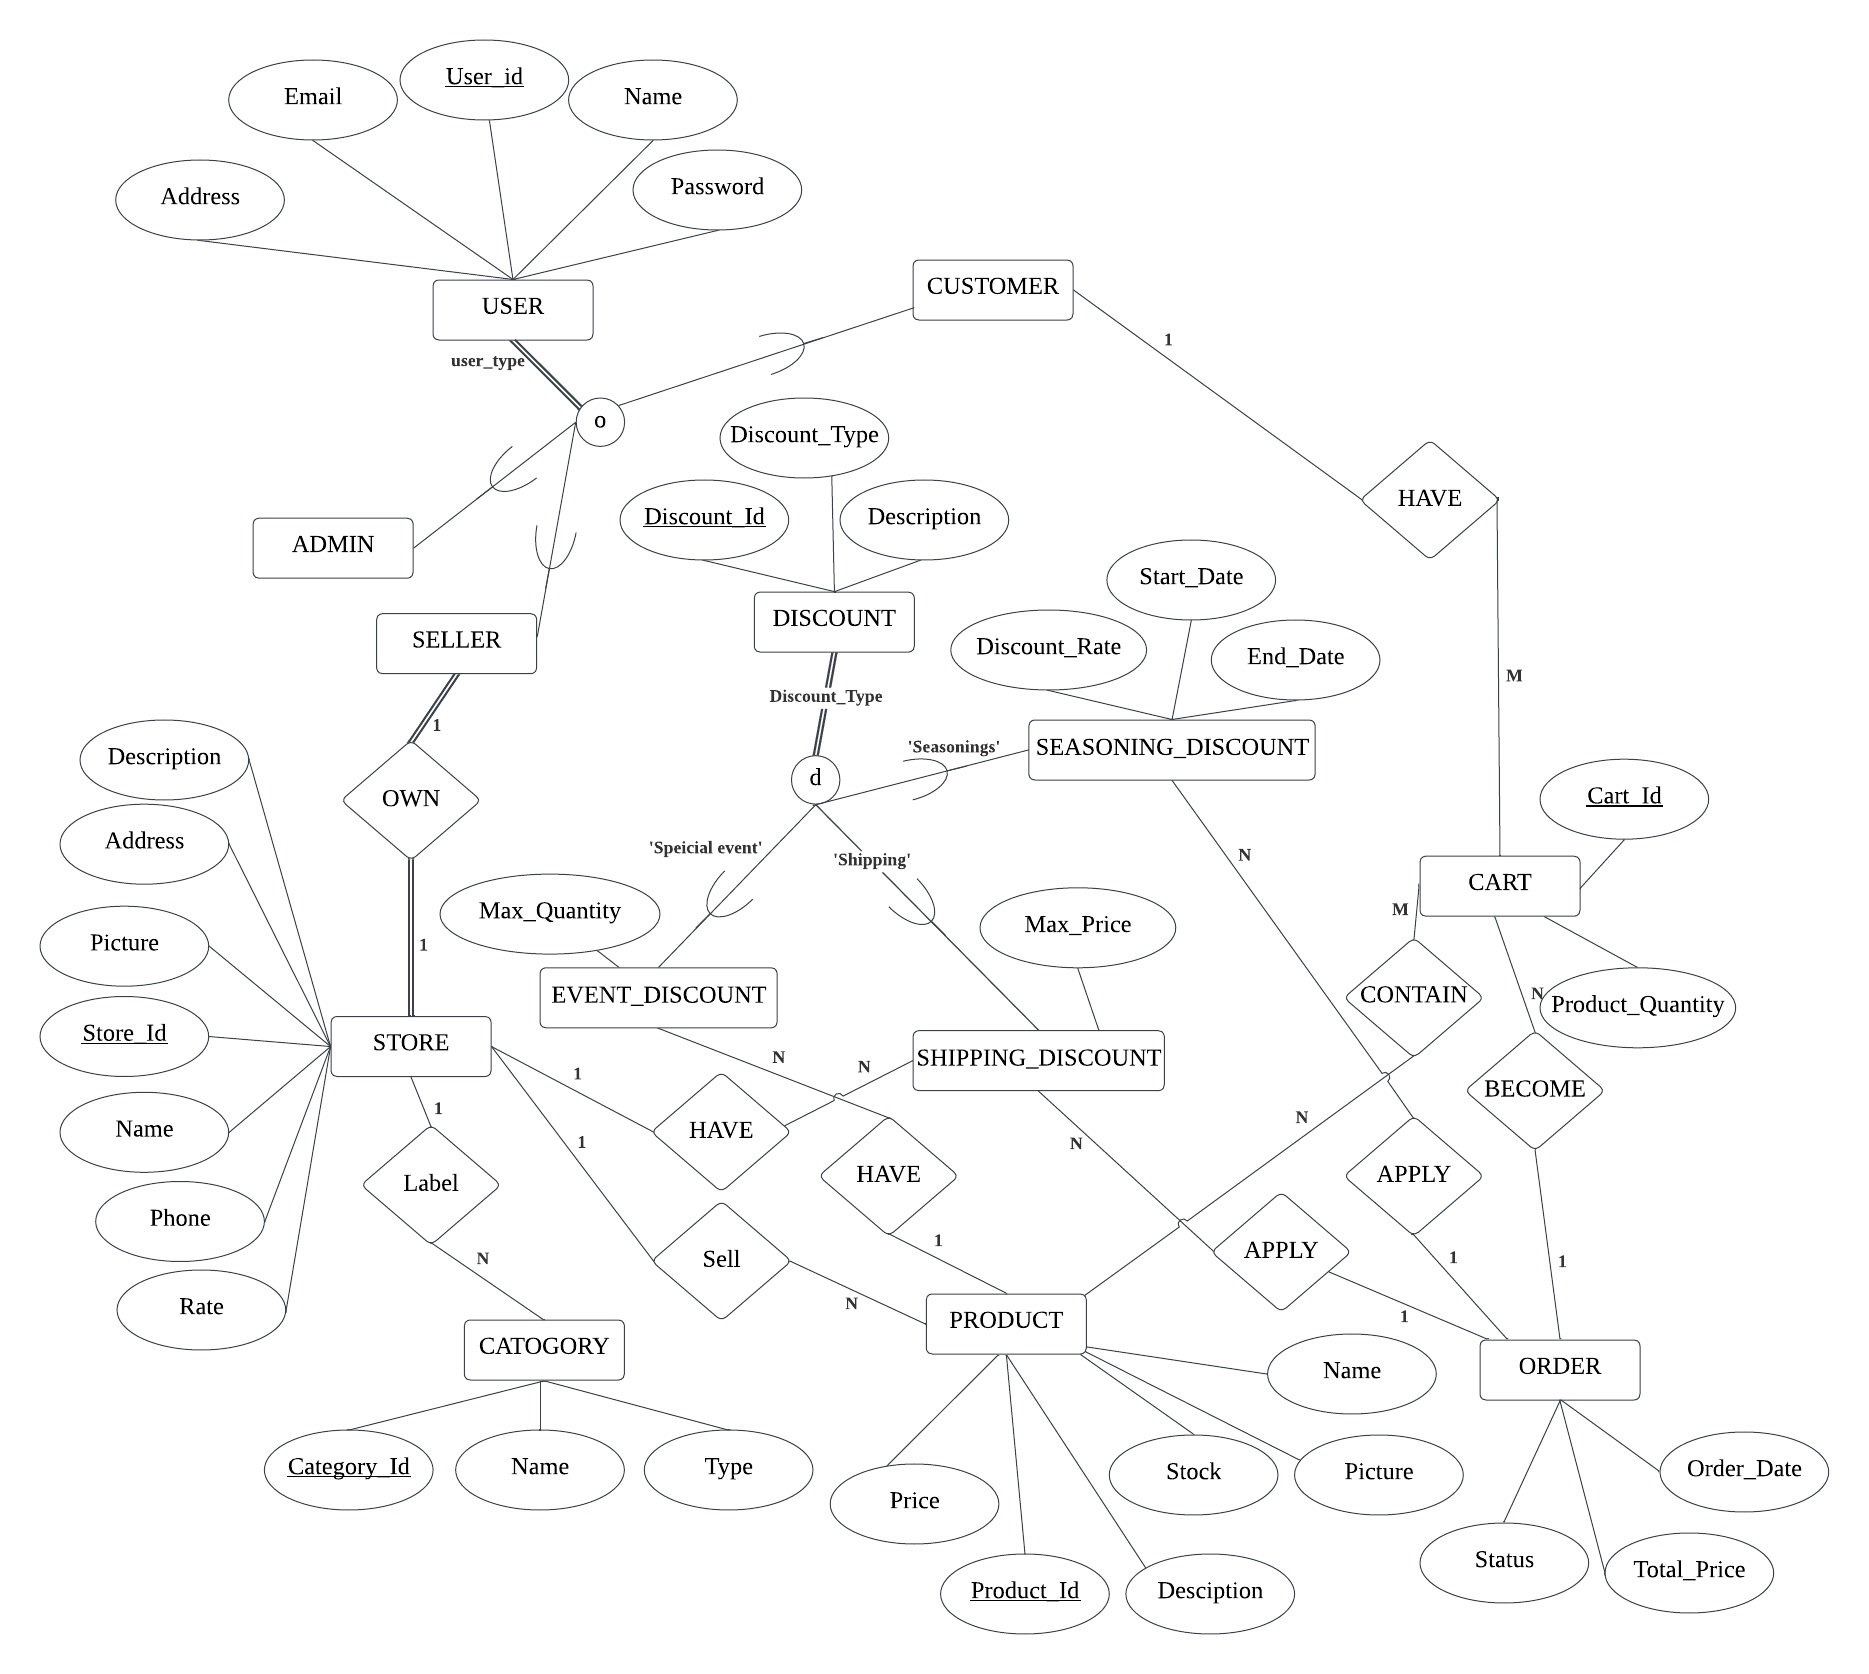
\includegraphics[width=40em]{ER-diagram.png}}
    \caption{ER diagram}
    \label{fig:enter-label}
\end{figure*}

\newpage

\section{Logical Database Schema}
\subsection{Schema of the Database}

\begin{figure*}[h]
    \centerline{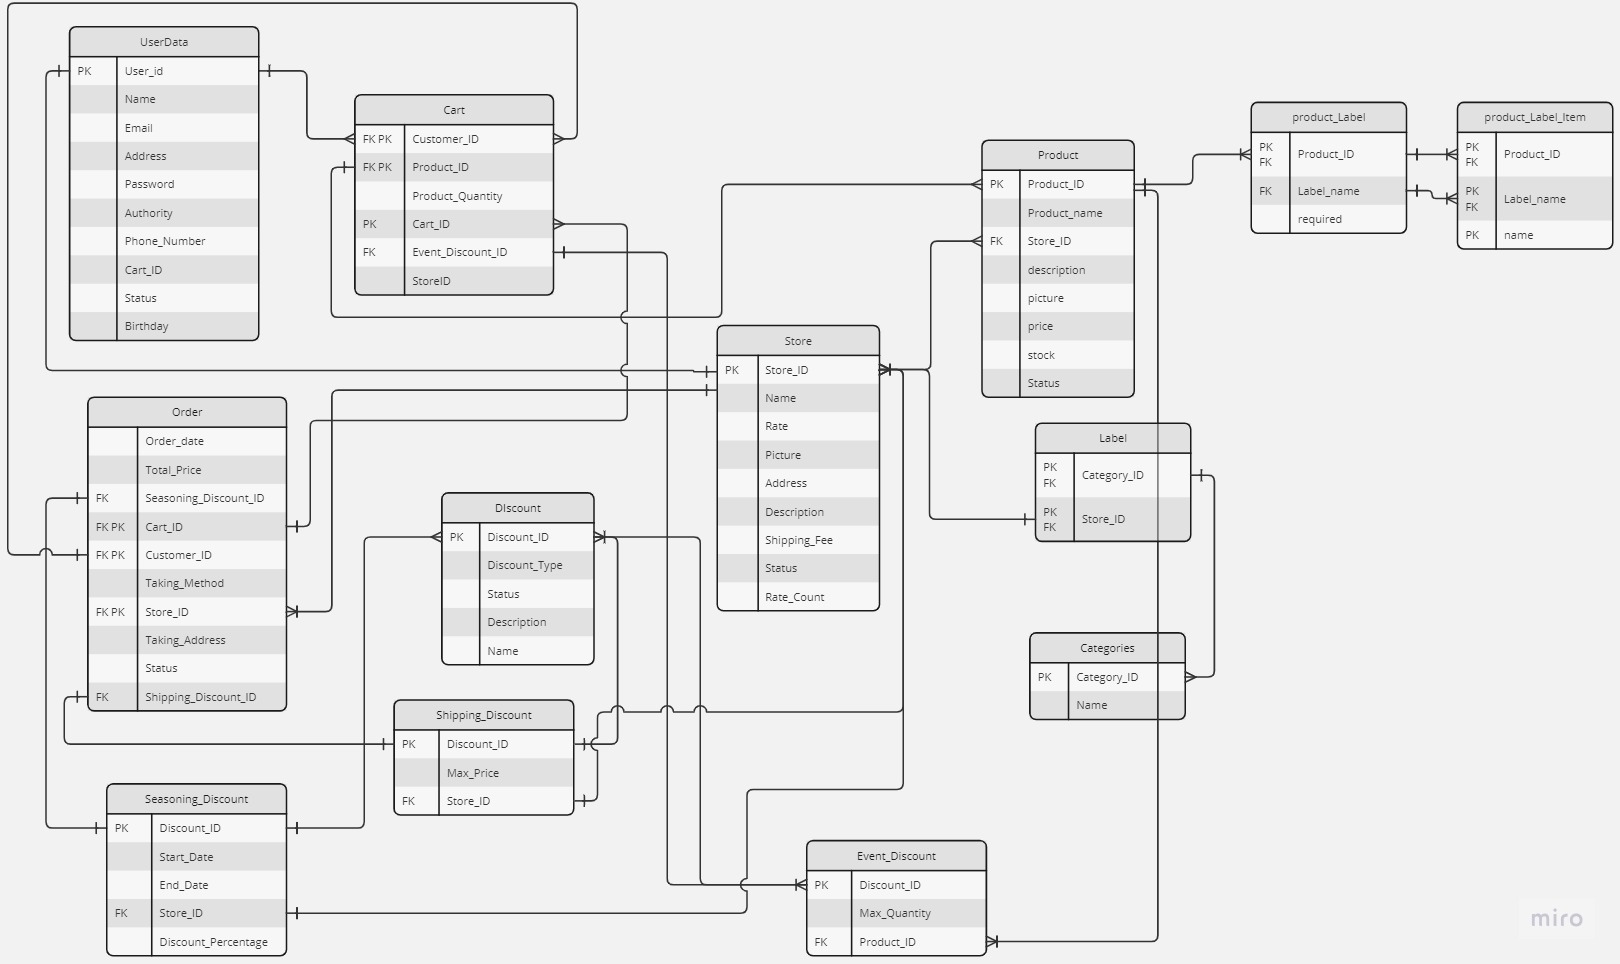
\includegraphics[width=40em]{schema-diagram.jpg}}    
    \caption{database schema}
    \label{fig:enter-label}
\end{figure*}

\newpage
\subsection{Data Dictionary}
%User
\noindent\begin{tabular}{ | p{7em} | p{5.5em} |p{5.5em} | p{4.5em} | p{11em} |}
  \hline
  \multicolumn{5}{|c|}{USER_DATA} \tabularnewline
  \hline 
  \multicolumn{5}{|c|}{Description: 使用者相關資料} \tabularnewline
  \hline 
  Attribute & Type & Key & Nullable & Description \\
  \hline
  user_id & SERIAL & Primary & Not Null & 使用者ID \\
  \hline
  name & VARCHAR & &Not Null &使用者名稱\\
  \hline
  email & VARCHAR & &Not Null &使用者信箱\\
  \hline
  address & VARCHAR & &Not Null &使用者地址\\
  \hline
  password & VARCHAR & &Not Null &使用者密碼\\
  \hline
  authority & INTEGER & &Not Null&\makecell[l]{使用者權限\\(admin, seller, user)} \\
  \hline
  phone_number & VARCHAR & &Not Null &使用者電話號碼\\
  \hline
  current_cart_id & INTEGER & &Not Null &使用者目前購物車\\
  \hline
  status & INTEGER & & Not Null & \makecell[l]{使用者狀態\\(0=停用, 1=啟用)}\\
  \hline
  birthday & DATE & & Not Null &使用者生日\\
  \hline
\end{tabular}
\vspace{1em}

%Cart
\noindent\begin{tabular}{ | p{7em} | p{5.5em} |p{5.5em} | p{4.5em} | p{11em} |}
  \hline
  \multicolumn{5}{|c|}{CARTS} \tabularnewline
  \hline 
  \multicolumn{5}{|c|}{Description: 購物車相關資料} \tabularnewline
  \hline 
  Attribute & Type & Key & Nullable & Description \\
  \hline
  customer_id& SERIAL & \makecell[l]{Primary \\ Foreign}  & Not Null & 使用者ID \\
  \hline
  product_id & SERIAL &\makecell[l]{Primary \\ Foreign} &Not Null &商品ID\\
  \hline
  cart_id & INTEGER &\makecell[l]{Primary}  &Not Null &購物車ID\\
  \hline
  product_quantity & INTEGER & &Not Null &商品數量\\
  \hline
  event_discount_id & SERIAL & Foreign &Not Null &折價券ID\\
  \hline
  store_id & SERIAL & \makecell[l]{Primary\\ Foreign} & Not Null & 購買商店ID\\
  \hline
\end{tabular}
\vspace{1em}

% %Product
\noindent\begin{tabular}{ | p{7em} | p{5.5em} | p{5.5em} | p{4.5em} | p{11em} |}
  \hline
  \multicolumn{5}{|c|}{PRODUCTS} \tabularnewline
  \hline 
  \multicolumn{5}{|c|}{Description: 商品相關資料} \tabularnewline
  \hline 
  Attribute & Type & Key & Nullable & Description \\
  \hline
  product_id& SERIAL & \makecell[l]{Primary \\ Foreign}  & Not Null & 商品ID \\
  \hline
  name & VARCHAR & &Not Null &商品名字\\
  \hline
  description & TEXT & &Not Null &商品資訊\\
  \hline
  store_id & SERIAL &Foreign &Not Null &商店ID\\
  \hline
  picture & STRING & &Not Null &商品照片\\
  \hline
  price & INTEGER & &Not Null &商品價錢\\
  \hline
  stock & INTEGER &  &Not Null &商品庫存\\
  \hline
  status & INTEGER &  &Not Null &\makecell[l]{商品狀態\\(0=停用,\\ 1=啟用,\\ 2=已售完)}\\
  \hline
\end{tabular}
\vspace{1em}

% %Store
\noindent\begin{tabular}{ | p{7em} | p{5.5em} | p{5.5em} | p{4.5em} | p{11em} |}
  \hline
  \multicolumn{5}{|c|}{STORES} \tabularnewline
  \hline 
  \multicolumn{5}{|c|}{Description: 商店相關資料} \tabularnewline
  \hline 
  Attribute & Type & Key & Nullable & Description \\
  \hline
  store_id& SERIAL & Primary & Not Null & 商品ID \\
  \hline
  name & VARCHAR & &Not Null &商店名字\\
  \hline
  rate & FLOAT & &Not Null &商店評價\\
  \hline
  picture & STRING & &Not Null &商店照片\\
  \hline
  address & VARCHAR & &Not Null &商店地址\\
  \hline
  description & TEXT & &Not Null &商店描述\\
  \hline
  shipping_fee & INTEGER & &Not Null &運費\\
  \hline
  status & INTEGER & &Not Null &\makecell[l]{商店狀態\\(0=停用, 1=啟用)}\\
  \hline
  rate_count & INTEGER & &Not Null &評價數量\\
  \hline
\end{tabular}
\vspace{1em}

%Label
\noindent\begin{tabular}{ | p{7em} | p{5.5em} | p{5.5em} | p{4.5em} | p{11em} |}
  \hline
  \multicolumn{5}{|c|}{LABEL} \tabularnewline
  \hline 
  \multicolumn{5}{|c|}{Description: 商店標籤資料} \tabularnewline
  \hline 
  Attribute & Type & Key & Nullable & Description \\
  \hline
  store_id& SERIAL & \makecell[l]{Primary \\ Foreign}& Not Null & 商店ID \\
  \hline
  category_id & SERIAL & \makecell[l]{Primary \\ Foreign} &Not Null &目錄ID\\
  \hline
\end{tabular}
\vspace{1em}

%Categories
\noindent\begin{tabular}{ | p{7em} | p{5.5em} | p{5.5em} | p{4.5em} | p{11em} |}
  \hline
  \multicolumn{5}{|c|}{CATEGORIES} \tabularnewline
  \hline 
  \multicolumn{5}{|c|}{Description: 類別資料} \tabularnewline
  \hline 
  Attribute & Type & Key & Nullable & Description \\
  \hline
  category_id& SERIAL & Primary & Not Null & 類別ID \\
  \hline
  name & VARCHAR & &Not Null &類別名稱\\
  \hline
\end{tabular}

\vspace{1em}
%enent_discount
\noindent\begin{tabular}{ | p{7em} | p{5.5em} | p{5.5em} | p{4.5em} | p{11em} |}
  \hline
  \multicolumn{5}{|c|}{EVENT_DISCOUNT} \tabularnewline
  \hline 
  \multicolumn{5}{|c|}{Description: 事件折扣資料} \tabularnewline
  \hline 
  Attribute & Type & Key & Nullable & Description \\
  \hline
  discount_id & SERIAL & Primary & Not Null & 折扣ID \\
  \hline
  max_quantity & INTEGER & &Not Null &買x送一\\
  \hline
  product_id & SERIAL & Foreign &Not Null &商品ID\\
  \hline
\end{tabular}
\vspace{1em}

%Shipping_discount
\noindent\begin{tabular}{ | p{7em} | p{5.5em} | p{5.5em} | p{4.5em} | p{11em} |}
  \hline
  \multicolumn{5}{|c|}{SHIPPING_DISCOUNT} \tabularnewline
  \hline 
  \multicolumn{5}{|c|}{Description: 運費折扣資料} \tabularnewline
  \hline 
  Attribute & Type & Key & Nullable & Description \\
  \hline
  discount_id & SERIAL & Primary & Not Null & 折扣ID \\
  \hline
  max_price & INTEGER & &Not Null &免運金額\\
  \hline
  store_id & SERIAL & Foreign &Not Null &商店ID\\
  \hline
\end{tabular}
\vspace{1em}

%Discount
\noindent\begin{tabular}{ | p{7em} | p{5.5em} | p{5.5em} | p{4.5em} | p{11em} |}
  \hline
  \multicolumn{5}{|c|}{DISCOUNTS} \tabularnewline
  \hline 
  \multicolumn{5}{|c|}{Description: 折扣資料} \tabularnewline
  \hline 
  Attribute & Type & Key & Nullable & Description \\
  \hline
  discount_id & SERIAL & Primary & Not Null & \makecell[l]{折扣ID\\1=無折扣} \\
  \hline
  discount_type & INTEGER &  & Not Null & \makecell[l]{折扣種類\\0=無折扣\\1=運費折扣\\2=季節性折扣\\3=事件折扣} \\
  \hline
  status & INTEGER & &Not Null &狀態\\
  \hline
  description& VARCHAR &  &Not Null &折價資訊\\
  \hline
  name & VARCHAR &  &Not Null &折扣名稱\\
  \hline
\end{tabular}
\vspace{1em}

%Order
\noindent\begin{tabular}{ | p{7em} | p{5.5em} | p{5.5em} | p{4.5em} | p{11em} |}
  \hline
  \multicolumn{5}{|c|}{ORDER} \tabularnewline
  \hline 
  \multicolumn{5}{|c|}{Description: 訂單} \tabularnewline
  \hline 
  Attribute & Type & Key & Nullable & Description \\
  \hline
  order_date & DATE &  & Not Null & 訂單日期 \\
  \hline
  total_price & INTEGER &  & Not Null & 總金額 \\
  \hline
  discount_id & SERIAL & Foreign&Not Null &折扣ID\\
  \hline
  cart_id& SERIAL & \makecell[l]{Primary \\ Foreign} &Not Null &購物車ID\\
  \hline
  customer_id & SERIAL & \makecell[l]{Primary \\ Foreign} & Not Null & 顧客ID \\
  \hline
  taking_method & INTEGER &  & Not Null &  \makecell[l]{0=自取\\1=外送}\\
  \hline
  store_id & SERIAL & \makecell[l]{Primary \\ Foreign} & Not Null & 商店ID \\
  \hline
  taking_address & VARCHAR &  & Not Null & 運送地址 \\
  \hline
  status & INTEGER &  & Not Null & \makecell[l]{訂單狀態\\0=未結帳\\1=已結帳\\2=接受訂單\\3=製作訂單\\4=運送中\\5=已送達\\6=確認訂單} \\
  \hline
  
  name & VARCHAR &  &Not Null &折扣名稱\\
  \hline
\end{tabular}


%Seasoning_discount
\noindent\begin{tabular}{ | p{7em} | p{5.5em} | p{5.5em} | p{4.5em} | p{11em} |}
  \hline
  \multicolumn{5}{|c|}{SEASONING_DISCOUNT} \tabularnewline
  \hline 
  \multicolumn{5}{|c|}{Description: 季節折扣資料} \tabularnewline
  \hline 
  Attribute & Type & Key & Nullable & Description \\
  \hline
  discount_id & SERIAL & Primary & Not Null & 折扣ID \\
  \hline
  start_date & DATE &  & Not Null & 開始日期 \\
  \hline
  end_date & DATE & &Not Null &結束日期\\
  \hline
  store_id& SERIAL & Foreign &Not Null &商店ID\\
  \hline
  discount_percentage & INTEGER &  &Not Null &\makecell[l]{折扣比例\\(70=30\%off)}\\
  \hline
\end{tabular}

%product_label
\noindent\begin{tabular}{ | p{7em} | p{5.5em} | p{5.5em} | p{4.5em} | p{11em} |}
  \hline
  \multicolumn{5}{|c|}{PRODUCT_LABEL} \tabularnewline
  \hline 
  \multicolumn{5}{|c|}{Description: 商品標籤} \tabularnewline
  \hline 
  Attribute & Type & Key & Nullable & Description \\
  \hline
  product_id & SERIAL & \makecell[l]{Primary \\ Foreign} & Not Null & 商品ID \\
  \hline
  label_name & VARCHAR & \makecell[l]{Primary \\ Foreign} & Not Null & 類別名稱 \\
  \hline
  required & BOOLEAN & & Not Null & 是否為必填\\
  \hline
\end{tabular}

%product_label_item
\noindent\begin{tabular}{ | p{7em} | p{5.5em} | p{5.5em} | p{4.5em} | p{11em} |}
  \hline
  \multicolumn{5}{|c|}{PRODUCT_LABEL_ITEM} \tabularnewline
  \hline 
  \multicolumn{5}{|c|}{Description: 商品標籤選項} \tabularnewline
  \hline 
  Attribute & Type & Key & Nullable & Description \\
  \hline
  product_id & SERIAL & \makecell[l]{Primary \\ Foreign} & Not Null & 商品ID \\
  \hline
  label_name & VARCHAR & \makecell[l]{Primary \\ Foreign} & Not Null & 類別名稱 \\
  \hline
  name & VARCHAR & Primary & Not Null & 選項名稱\\
  \hline
\end{tabular}

\newpage

\subsection{Snapshot of Tables}
\begin{figure}[hp]
    \centerline{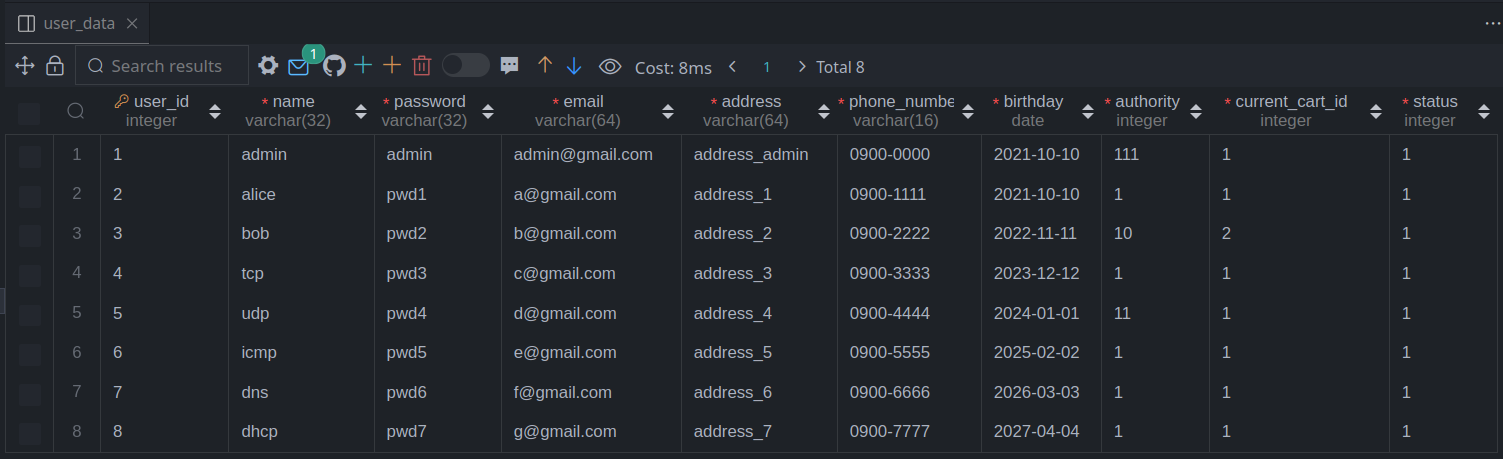
\includegraphics[width=\linewidth]{snapshot/user_data.png}}
    \caption{user_data}
\end{figure}


\begin{figure}[hp]
    \centerline{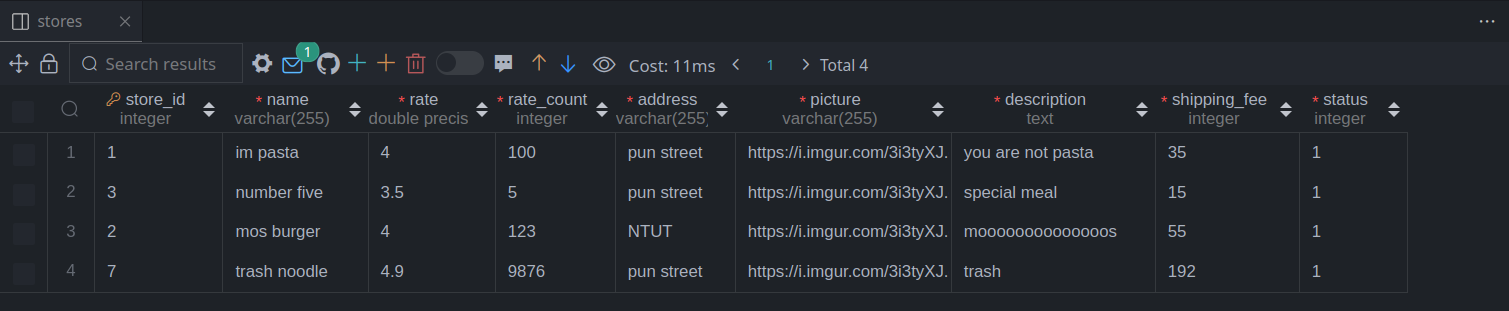
\includegraphics[width=\linewidth]{snapshot/stores.png}}
    \caption{stores}
\end{figure}

\begin{figure}[hp]
    \centerline{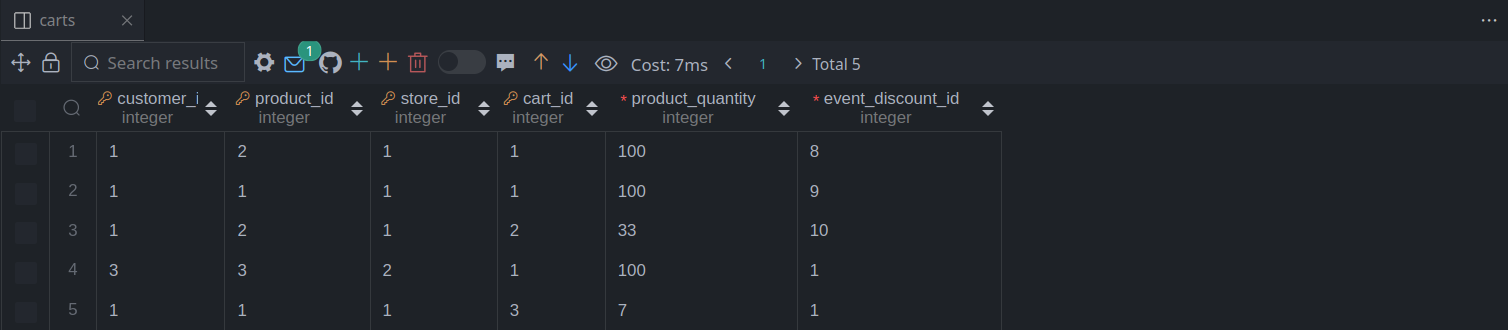
\includegraphics[width=\linewidth]{snapshot/carts.png}}
    \caption{carts}
\end{figure}

\begin{figure}[hp]
    \centerline{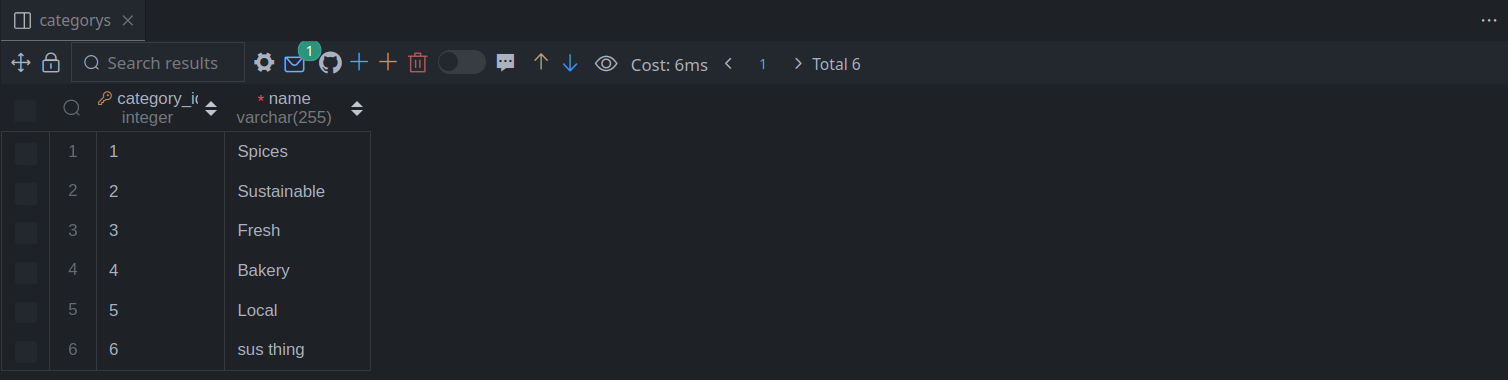
\includegraphics[width=\linewidth]{snapshot/categories.png}}
    \caption{categories}
\end{figure}

\begin{figure}[hp]
    \centerline{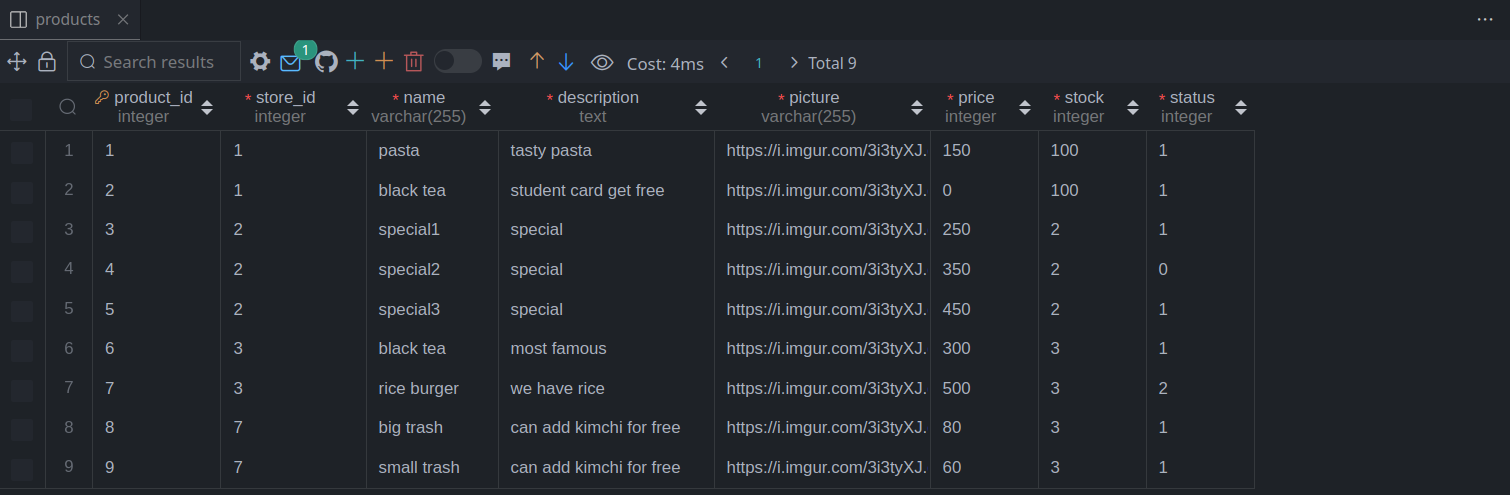
\includegraphics[width=\linewidth]{snapshot/products.png}}
    \caption{products}
\end{figure}

\begin{figure}[hp]
    \centerline{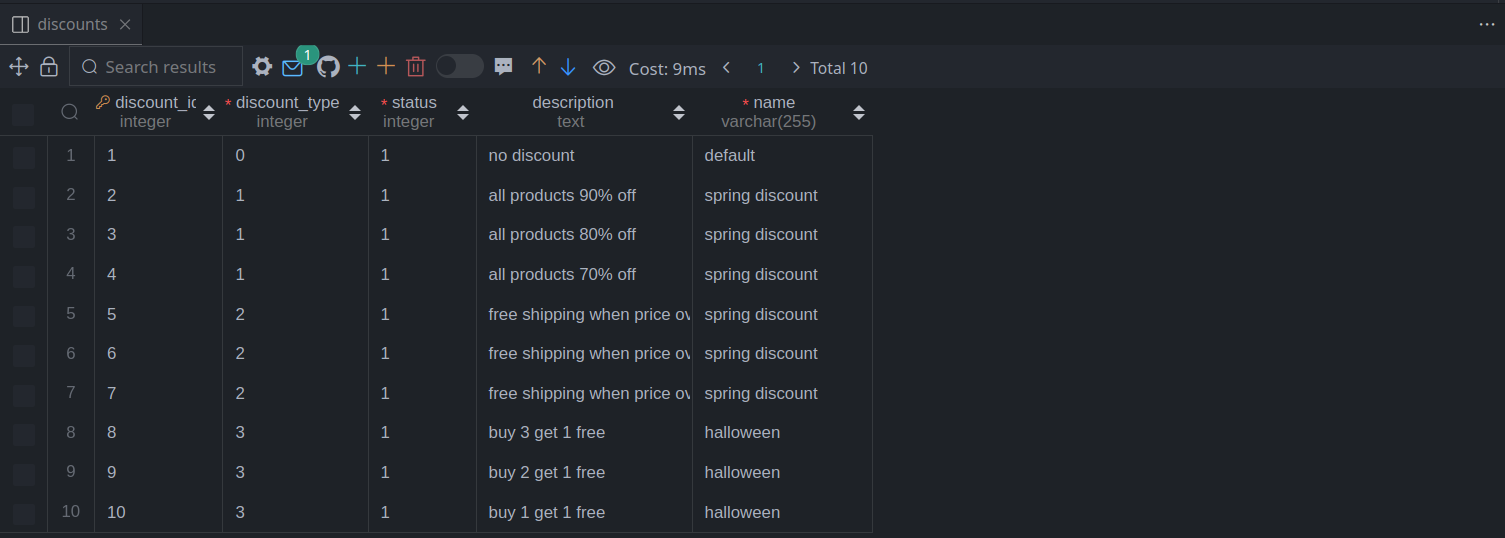
\includegraphics[width=\linewidth]{snapshot/discounts.png}}
    \caption{discounts}
\end{figure}

\begin{figure}[hp]
    \centerline{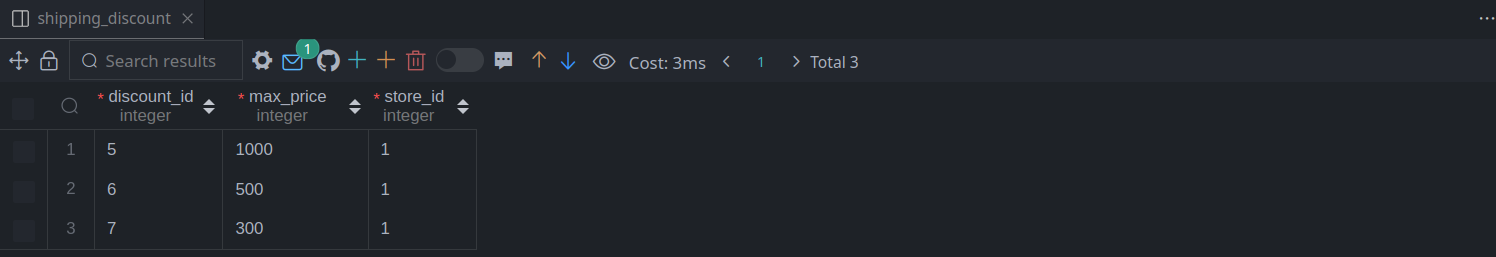
\includegraphics[width=\linewidth]{snapshot/shipping_discount.png}}
    \caption{shipping_discount}
\end{figure}

\begin{figure}[hp]
    \centerline{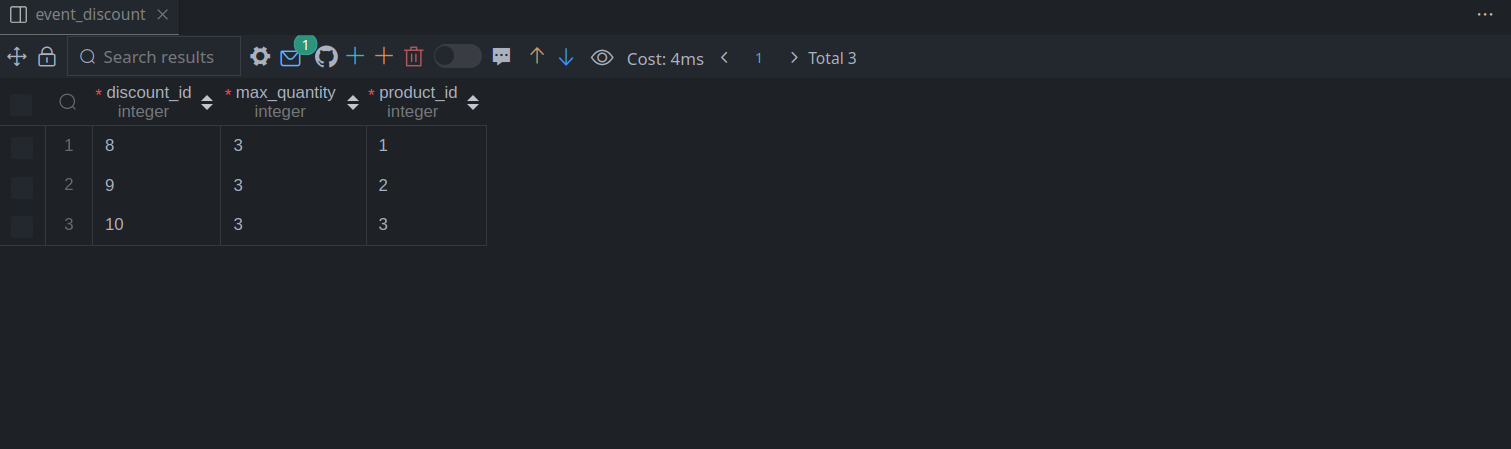
\includegraphics[width=\linewidth]{snapshot/event_discount.png}}
    \caption{event_discount}
\end{figure}

\begin{figure}[hp]
    \centerline{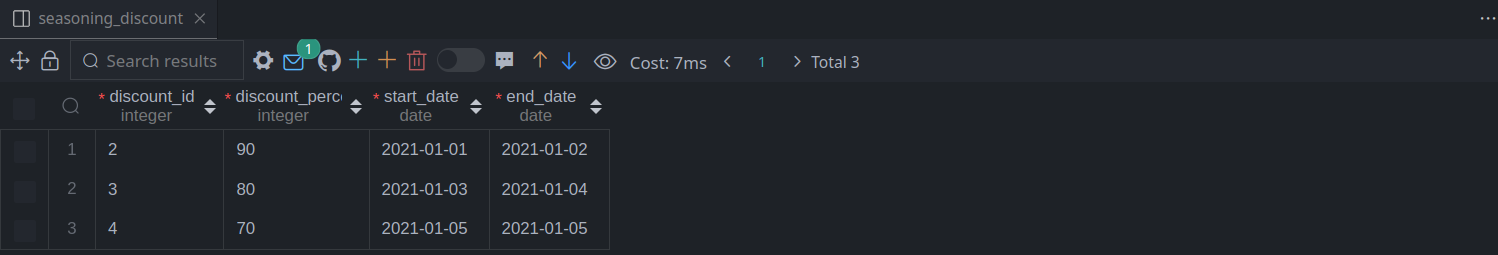
\includegraphics[width=\linewidth]{snapshot/seasoning_discount.png}}
    \caption{seasoning_discount}
\end{figure}

\begin{figure}[hp]
    \centerline{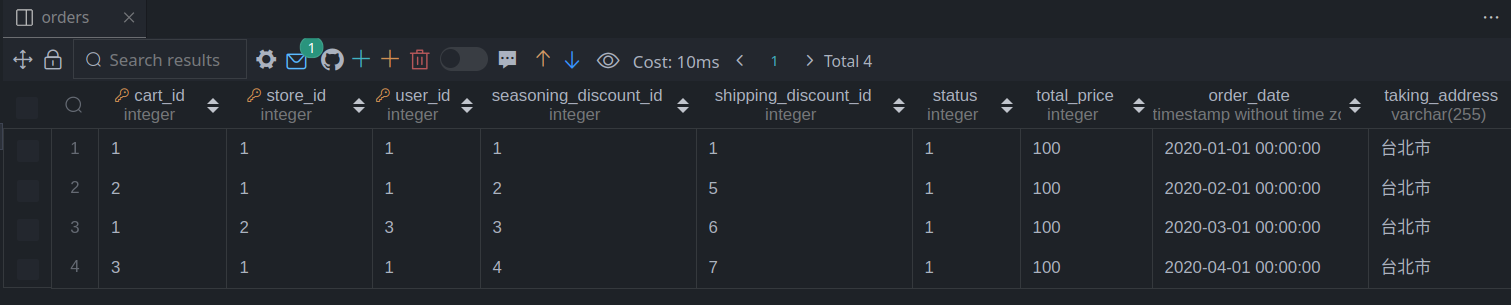
\includegraphics[width=\linewidth]{snapshot/orders.png}}
    \caption{orders}
\end{figure}

\begin{figure}[hp]
    \centerline{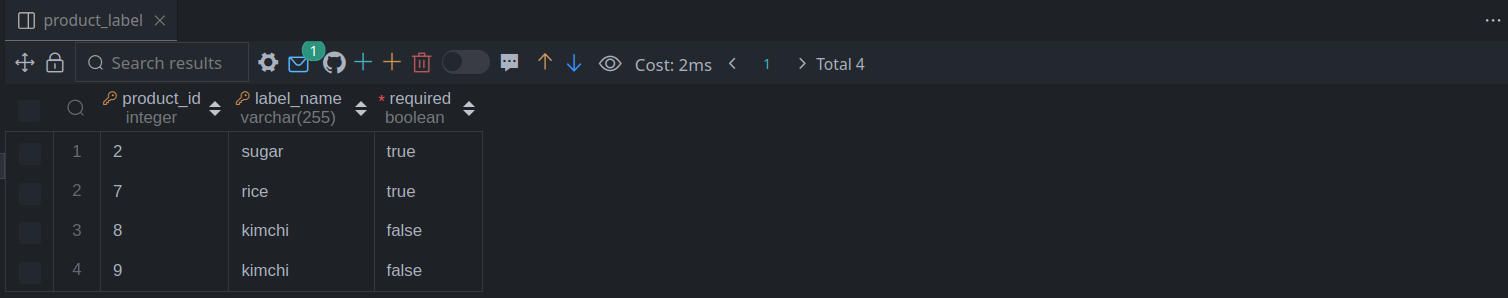
\includegraphics[width=\linewidth]{snapshot/product_label.png}}
    \caption{product_label}
\end{figure}

\begin{figure}[hp]
    \centerline{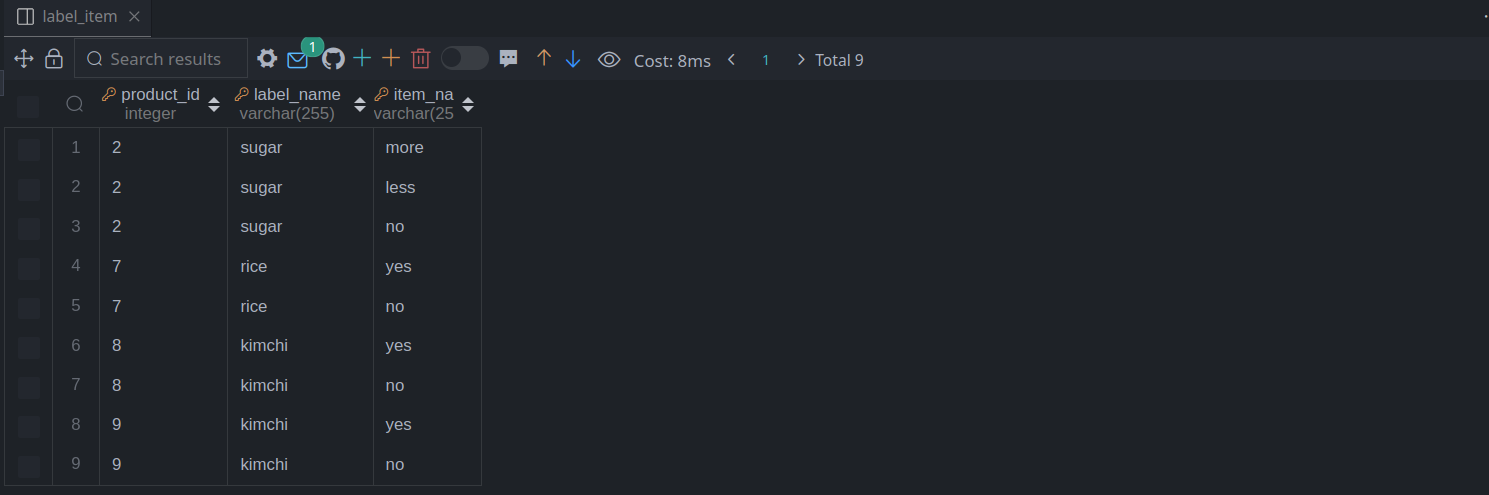
\includegraphics[width=\linewidth]{snapshot/label_item.png}}
    \caption{label_item}
\end{figure}

\clearpage

\begin{figure}[h!]
    \centerline{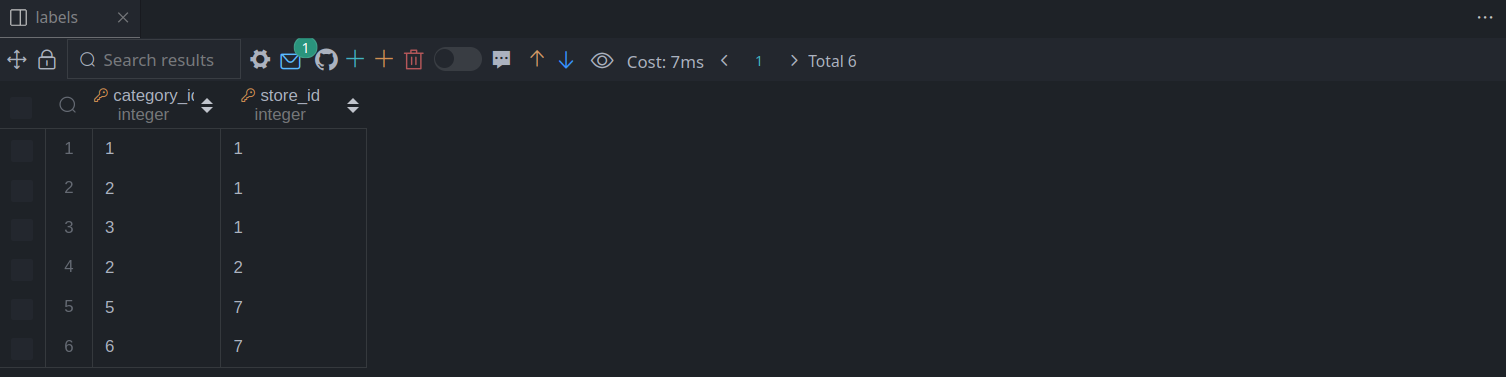
\includegraphics[width=\linewidth]{snapshot/labels.png}}
    \caption{labels}
\end{figure}

\clearpage

\subsection{SQL Statements for Database Construction}
\subsubsection{Create Table}
\begin{lstlisting}
-- user_data
CREATE TABLE
    IF NOT EXISTS user_data(
        user_id SERIAL PRIMARY KEY,
        name VARCHAR(32) NOT NULL,
        password VARCHAR(32) NOT NULL,
        email VARCHAR(64) UNIQUE NOT NULL,
        address VARCHAR(64) NOT NULL,
        phone_number VARCHAR(16) NOT NULL,
        birthday DATE NOT NULL,
        authority INTEGER NOT NULL,
        current_cart_id INTEGER NOT NULL,
        status INTEGER NOT NULL
    );
\end{lstlisting}

\begin{lstlisting}
-- stores
CREATE TABLE
    IF NOT EXISTS stores (
        store_id SERIAL PRIMARY KEY REFERENCES user_data(user_id),
        name VARCHAR(255) NOT NULL,
        rate FLOAT NOT NULL,
        rate_count INTEGER NOT NULL,
        address VARCHAR(255) NOT NULL,
        picture VARCHAR(255) NOT NULL,
        description TEXT NOT NULL,
        shipping_fee INTEGER NOT NULL,
        status INTEGER NOT NULL
    );
\end{lstlisting}

\begin{lstlisting}
-- products
CREATE TABLE
    IF NOT EXISTS products (
        product_id SERIAL PRIMARY KEY,
        store_id SERIAL REFERENCES stores(store_id),
        name VARCHAR(255) NOT NULL,
        description TEXT NOT NULL,
        picture VARCHAR(255) NOT NULL,
        price INTEGER NOT NULL,
        stock INTEGER NOT NULL,
        status INTEGER NOT NULL
    );
\end{lstlisting}

\begin{lstlisting}
-- discounts
CREATE TABLE
    IF NOT EXISTS discounts (
        discount_id SERIAL PRIMARY KEY UNIQUE,
        discount_type INT NOT NULL,
        status INT NOT NULL,
        description TEXT,
        name VARCHAR(255) NOT NULL
    );
\end{lstlisting}

\begin{lstlisting}
-- seasoning_discount
CREATE TABLE
    IF NOT EXISTS seasoning_discount (
        discount_id SERIAL UNIQUE REFERENCES discounts(discount_id),
        discount_percentage INT NOT NULL,
        start_date DATE NOT NULL,
        end_date DATE NOT NULL
    );
\end{lstlisting}

\begin{lstlisting}
-- shopping_discount
CREATE TABLE
    IF NOT EXISTS shipping_discount (
        discount_id SERIAL UNIQUE REFERENCES discounts(discount_id),
        max_price INT NOT NULL,
        store_id SERIAL REFERENCES stores(store_id)
    );
\end{lstlisting}

\begin{lstlisting}
-- event_discount
CREATE TABLE
    IF NOT EXISTS event_discount (
        discount_id SERIAL UNIQUE REFERENCES discounts(discount_id),
        max_quantity INT NOT NULL,
        product_id SERIAL REFERENCES products(product_id)
    );
\end{lstlisting}

\begin{lstlisting}
-- carts
CREATE TABLE
    IF NOT EXISTS carts (
        customer_id SERIAL REFERENCES user_data(user_id),
        product_id SERIAL REFERENCES products(product_id),
        store_id SERIAL REFERENCES stores(store_id),
        cart_id INTEGER NOT NULL,
        product_quantity INT NOT NULL,
        event_discount_id SERIAL REFERENCES discounts(discount_id),
        PRIMARY KEY (
            customer_id,
            product_id,
            store_id,
            cart_id
        )
    );
\end{lstlisting}

\begin{lstlisting}
-- orders
CREATE TABLE
    orders (
        cart_id INTEGER,
        store_id INTEGER REFERENCES stores(store_id),
        user_id INTEGER REFERENCES user_data(user_id),
        seasoning_discount_id INTEGER REFERENCES discounts(discount_id),
        shipping_discount_id INTEGER REFERENCES discounts(discount_id),
        status INTEGER,
        total_price INTEGER,
        Order_date TIMESTAMP,
        taking_address VARCHAR(255),
        taking_method INTEGER,
        PRIMARY KEY (cart_id, store_id, user_id)
    );
\end{lstlisting}

\begin{lstlisting}
-- categories
CREATE TABLE
    IF NOT EXISTS categories (
        category_id SERIAL PRIMARY KEY,
        name VARCHAR(255) UNIQUE NOT NULL
    );
\end{lstlisting}

\begin{lstlisting}
-- product_label
CREATE TABLE
    IF NOT EXISTS product_label (
        product_id SERIAL REFERENCES products(product_id),
        label_name VARCHAR(255) NOT NULL,
        required BOOLEAN NOT NULL,
        PRIMARY KEY (product_id, label_name)
    );
\end{lstlisting}

\begin{lstlisting}
-- label_item
CREATE TABLE
    IF NOT EXISTS label_item (
        product_id SERIAL NOT NULL,
        label_name VARCHAR(255) NOT NULL,
        item_name VARCHAR(255) NOT NULL,
        FOREIGN KEY (product_id, label_name) REFERENCES product_label(product_id, label_name),
        PRIMARY KEY (product_id, label_name, item_name)
    );
\end{lstlisting}

\subsubsection{Insert Data}

\begin{lstlisting}
-- user_data
INSERT INTO user_data (name, password, email, address, phone_number, birthday, authority, current_cart_id, status) VALUES
    ('admin', 'admin', 'admin@gmail.com', 'address_admin', '0900-0000', '2021-10-10 11:30:30', 111, 1, 1),
    ('alice', 'pwd1', 'a@gmail.com', 'address_1', '0900-1111', '2021-10-10 11:30:30', 001, 1, 1),
    ('bob', 'pwd2', 'b@gmail.com', 'address_2', '0900-2222', '2022-11-11 11:30:30', 010, 2, 1),
    ('tcp', 'pwd3', 'c@gmail.com', 'address_3', '0900-3333', '2023-12-12 11:30:30', 001, 1, 1),
    ('udp', 'pwd4', 'd@gmail.com', 'address_4', '0900-4444', '2024-01-01 11:30:30', 011, 1, 1),
    ('icmp', 'pwd5', 'e@gmail.com', 'address_5', '0900-5555', '2025-02-02 11:30:30', 001, 1, 1),
    ('dns', 'pwd6', 'f@gmail.com', 'address_6', '0900-6666', '2026-03-03 11:30:30', 001, 1, 1),
    ('dhcp', 'pwd7', 'g@gmail.com', 'address_7', '0900-7777', '2027-04-04 11:30:30', 001, 1, 1);
\end{lstlisting}

\begin{lstlisting}
-- stores
INSERT INTO stores (store_id, name, rate, rate_count, address, picture, description, shipping_fee, status) VALUES 
    (1, 'im pasta', 4, 100, 'pun street', 'https://i.imgur.com/3i3tyXJ.gif', 'you are not pasta', 35, 1),
    (3, 'number five',3.5, 5, 'pun street', 'https://i.imgur.com/3i3tyXJ.gif', 'special meal', 15, 1),
    (2, 'mos burger',4, 123, 'NTUT', 'https://i.imgur.com/3i3tyXJ.gif', 'moooooooooooooos', 55, 1),
    (7, 'trash noodle',4.9, 9876, 'pun street', 'https://i.imgur.com/3i3tyXJ.gif', 'trash', 192, 1);
\end{lstlisting}

\begin{lstlisting}
-- products
INSERT INTO products (store_id, name, description, picture, price, stock, status) VALUES
    (1, 'pasta', 'tasty pasta', 'https://i.imgur.com/3i3tyXJ.gif', 150, 100, 1),
    (1, 'black tea', 'student card get free', 'https://i.imgur.com/3i3tyXJ.gif', 0, 100, 1),
    (2, 'special1', 'special', 'https://i.imgur.com/3i3tyXJ.gif', 250, 2, 1),
    (2, 'special2', 'special', 'https://i.imgur.com/3i3tyXJ.gif', 350, 2, 0),
    (2, 'special3', 'special', 'https://i.imgur.com/3i3tyXJ.gif', 450, 2, 1),
    (3, 'black tea', 'most famous', 'https://i.imgur.com/3i3tyXJ.gif', 300, 3, 1),
    (3, 'rice burger', 'we have rice', 'https://i.imgur.com/3i3tyXJ.gif', 500, 3, 2),
    (7, 'big trash', 'can add kimchi for free', 'https://i.imgur.com/3i3tyXJ.gif', 80, 3, 1),
    (7, 'small trash', 'can add kimchi for free', 'https://i.imgur.com/3i3tyXJ.gif', 60, 3, 1);
\end{lstlisting}

\begin{lstlisting}
-- discounts
INSERT INTO discounts (discount_type, description, name, status) VALUES
(0, 'no discount', 'default', 1),
(1, 'all products 90% off', 'spring discount', 1),
(1, 'all products 80% off', 'spring discount', 1),
(1, 'all products 70% off', 'spring discount', 1),
(2, 'free shipping when price over 1000', 'spring discount', 1),
(2, 'free shipping when price over 500', 'spring discount', 1),
(2, 'free shipping when price over 300', 'spring discount', 1),
(3, 'buy 3 get 1 free', 'halloween', 1),
(3, 'buy 2 get 1 free', 'halloween', 1),
(3, 'buy 1 get 1 free', 'halloween', 1);
\end{lstlisting}

\begin{lstlisting}
-- seasoning_discount
INSERT INTO seasoning_discount (discount_id, discount_percentage, start_date, end_date) VALUES
    (2,90,'2021-01-01 00:00:00','2021-01-02 00:00:00'),
    (3,80,'2021-01-03 00:00:00','2021-01-04 00:00:00'),
    (4,70,'2021-01-05 00:00:00','2021-01-05 00:00:00');
\end{lstlisting}

\begin{lstlisting}
-- shipping_discount
INSERT INTO shipping_discount (discount_id, max_price, store_id) VALUES
  (5,1000,1),
  (6,500,1),
  (7,300,1);
\end{lstlisting}

\begin{lstlisting}
-- event_discount
INSERT INTO event_discount (discount_id, max_quantity, product_id) VALUES
    (8,3,1),
    (9,3,2),
    (10,3,3);
\end{lstlisting}

\begin{lstlisting}
-- carts
INSERT INTO carts (customer_id, cart_id, store_id, product_id, product_quantity, event_discount_id) VALUES
    (1, 1, 1, 2, 100, 8),
    (1, 1, 1, 1, 100, 9),
    (1, 2, 1, 2, 33, 10),
    (3, 1, 2, 3, 100, 1),
    (1, 3, 1, 1, 7, 1);
\end{lstlisting}

\begin{lstlisting}
-- orders
INSERT INTO orders (user_id, cart_id, store_id, seasoning_discount_id, shipping_discount_id, status, total_price, Order_date, taking_address, taking_method) VALUES 
    (1, 1, 1, 1, 1, 1, 100, '2020-01-01 00:00:00', '台北市', 1),
    (1, 2, 1, 2, 5, 1, 100, '2020-02-01 00:00:00', '台北市', 1),
    (3, 1, 2, 3, 6, 1, 100, '2020-03-01 00:00:00', '台北市', 1),
    (1, 3, 1, 4, 7, 1, 100, '2020-04-01 00:00:00', '台北市', 1);
\end{lstlisting}

\begin{lstlisting}
-- categories
INSERT INTO categories (name) VALUES
    ('Spices'),
    ('Sustainable'),
    ('Fresh'),
    ('Bakery'),
    ('Local'),
    ('sus thing');
\end{lstlisting}

\begin{lstlisting}
-- labels
INSERT INTO labels (category_id, store_id) VALUES
    (1, 1),
    (2, 1),
    (3, 1),
    (2, 2),
    (5, 7),
    (6, 7);
\end{lstlisting}

\begin{lstlisting}
-- product_label
INSERT INTO product_label (product_id, label_name, required) VALUES
    (2,'sugar', true),
    (7,'rice', true),
    (8, 'kimchi', false),
    (9, 'kimchi', false);
\end{lstlisting}

\begin{lstlisting}
-- label_item
INSERT INTO label_item (product_id, label_name, item_name) VALUES
    (2, 'sugar', 'more'),
    (2, 'sugar', 'less'),
    (2, 'sugar', 'no'),
    (7, 'rice', 'yes'),
    (7, 'rice', 'no'),
    (8, 'kimchi', 'yes'),
    (8, 'kimchi', 'no'),
    (9, 'kimchi', 'yes'),
    (9, 'kimchi', 'no');
\end{lstlisting}

\newpage

\subsection{Size of Each table}

\noindent\begin{tabular}{ | p{8em} | p{6.5em} | p{6.5em} | p{8em} |}
  \hline 
  Table & Tuple Size (bytes) & Average Tuple Count & Estimate Size (kb) \\
  \hline
  user_data & 92 & 300 & 27.6 \\
  \hline
  stores & 120 & 30 & 3.6 \\
  \hline
  products & 110 & 600 & 66 \\
  \hline
  carts & 50 & 4000 & 200 \\
  \hline
  discounts & 70 & 250 & 17.5 \\
  \hline
  seasoning_discount & 40 & 20 & 0.8 \\
  \hline
  shipping_discount & 40 & 30 & 1.2 \\
  \hline
  event_discount & 40 & 200 & 8 \\
  \hline
  orders & 80 & 1500 & 120 \\
  \hline
  categories & 40 & 10 & 0.4 \\
  \hline
  labels & 35 & 120 & 42 \\
  \hline
  product_label & 35 & 400 & 14 \\
  \hline
  label_item & 40 & 1200 & 48 \\
  \hline
\end{tabular}

\subsection{Expected Database Operation}

\noindent\begin{tabular}{ | p{12em} | p{9em} | p{9em} |}
  \hline 
  Table & 可能操作 & 頻率(次數/天)  \\
  \hline
  user_data 
        & 登入 & 150 \\
        & 註冊 & 5 \\
  \hline
  stores
        & 新增商店 & 2 \\
        & 查看商店資料 & 200 \\
        & 為商店評分 & 20 \\
        & 編輯商店 & 2 \\
  \hline
  products
        & 新增商品 & 2 \\
        & 查看商品資料 & 60 \\
        & 編輯商品 & 10 \\
  \hline
  carts
        & 加入購物車 & 250 \\
        & 結帳 & 90 \\
        & 查看購物車 & 100 \\
  \hline
  discounts 
        & 新增折扣 & 9 \\
        & 編輯折扣 & 3 \\
        & 查看折扣 & 100 \\
  \hline
  seasoning_discounts
        & 新增折扣 & 3 \\
        & 編輯折扣 & 1 \\
  \hline
  shipping_discount
        & 新增折扣 & 3 \\
        & 編輯折扣 & 1 \\
  \hline
  event_discount
        & 新增折扣 & 3 \\
        & 編輯折扣 & 1 \\
  \hline
  orders 
        & 查看訂單 & 100 \\
        & 更新訂單 & 400 \\
  \hline
  categories 
        & 查看類別 & 50 \\
  \hline
  labels 
        & 編輯店家類別 & 2 \\
  \hline
  product_label 
        & 新增商品類別 & 10 \\
        & 編輯商品類別 & 2 \\
  \hline
  label_item
        & 新增商品類別品項 & 30 \\
        & 編輯商品類別品項 & 10 \\
  \hline
\end{tabular}

\newpage

\section{Implementation and Demonstration of the Database System }

\subsection{Snapshots of GUI}
\begin{figure}[hp]
    \centerline{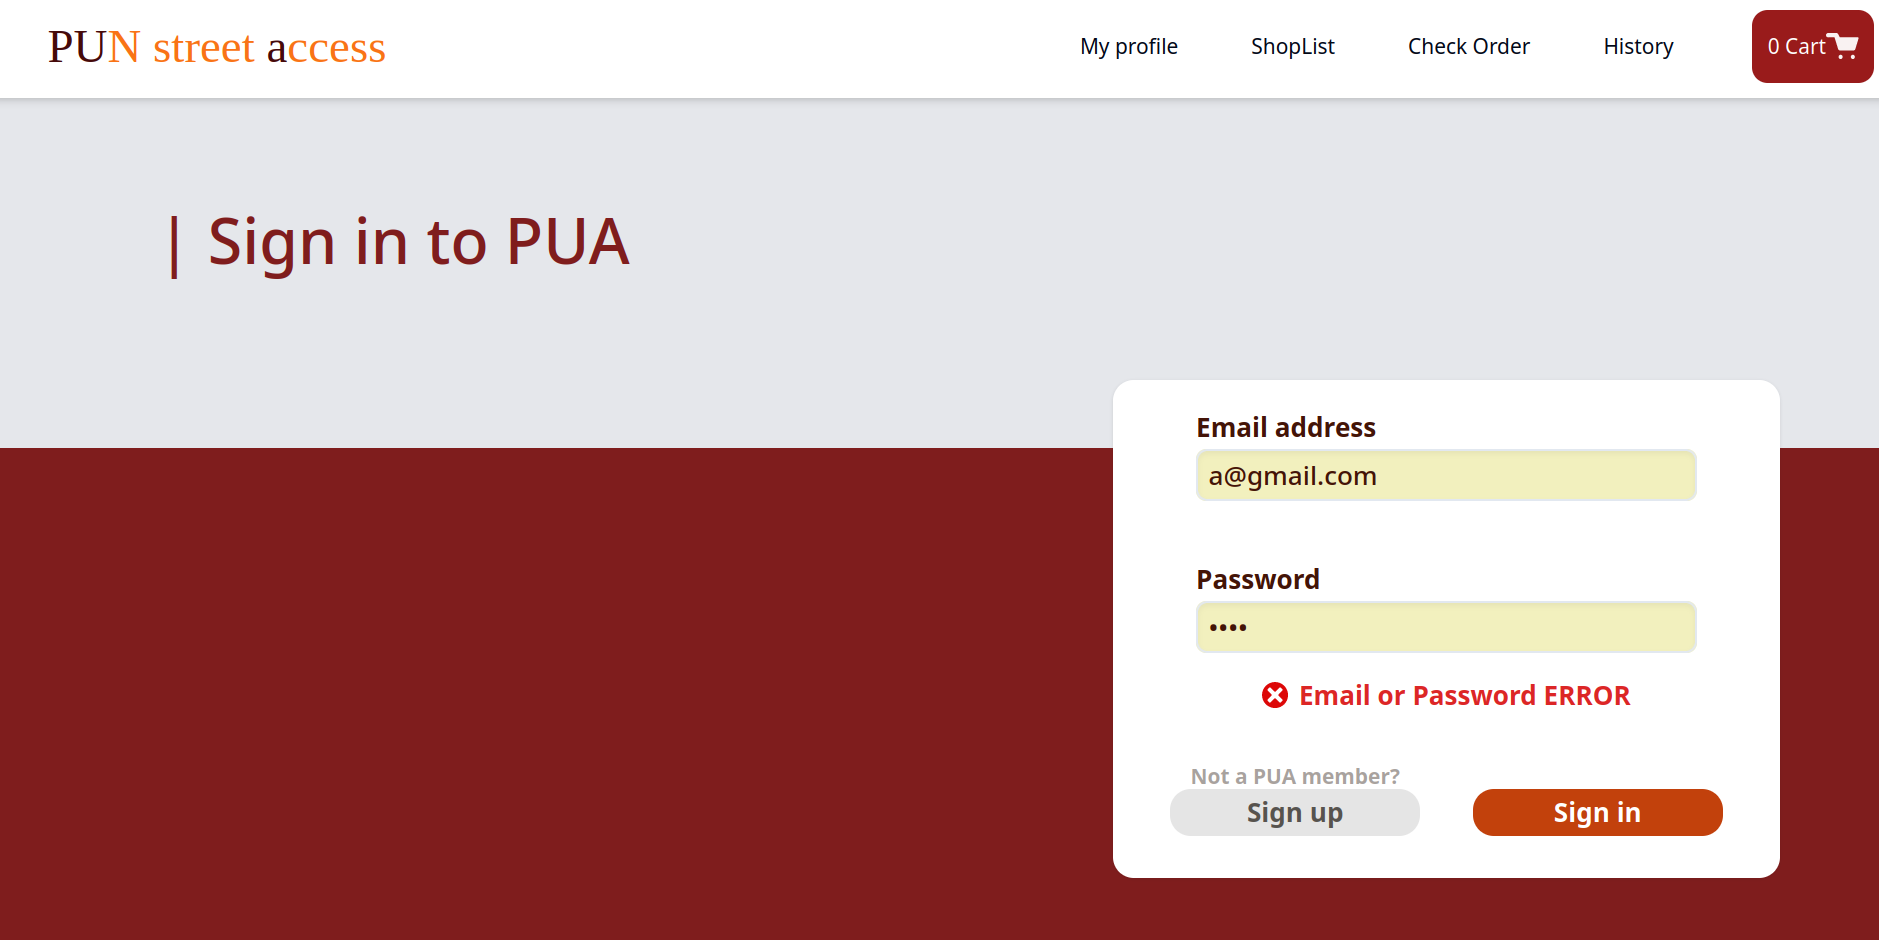
\includegraphics[width=40em]{pic/login.png}}
    \caption{login page}
    \label{fig:enter-label}
\end{figure}

\begin{figure}[hp]
    \centerline{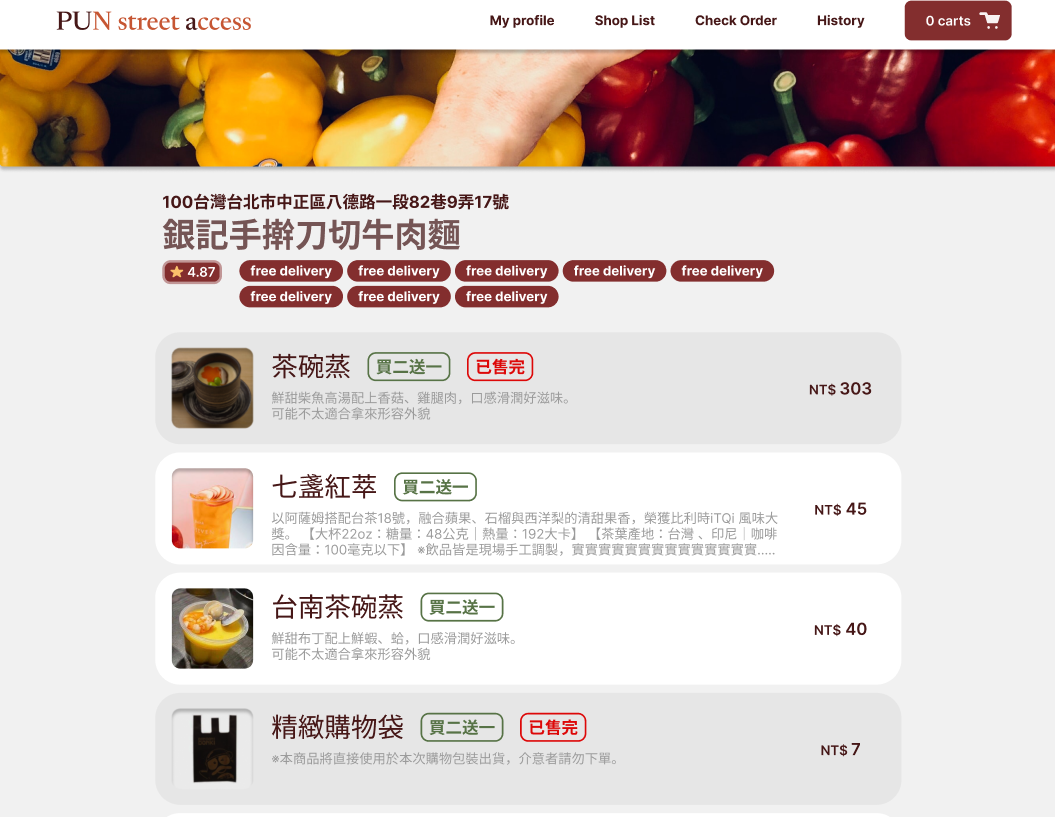
\includegraphics[width=40em]{pic/shop.png}}
    \caption{shop page}
    \label{fig:enter-label}
\end{figure}

\begin{figure}[hp]
    \centerline{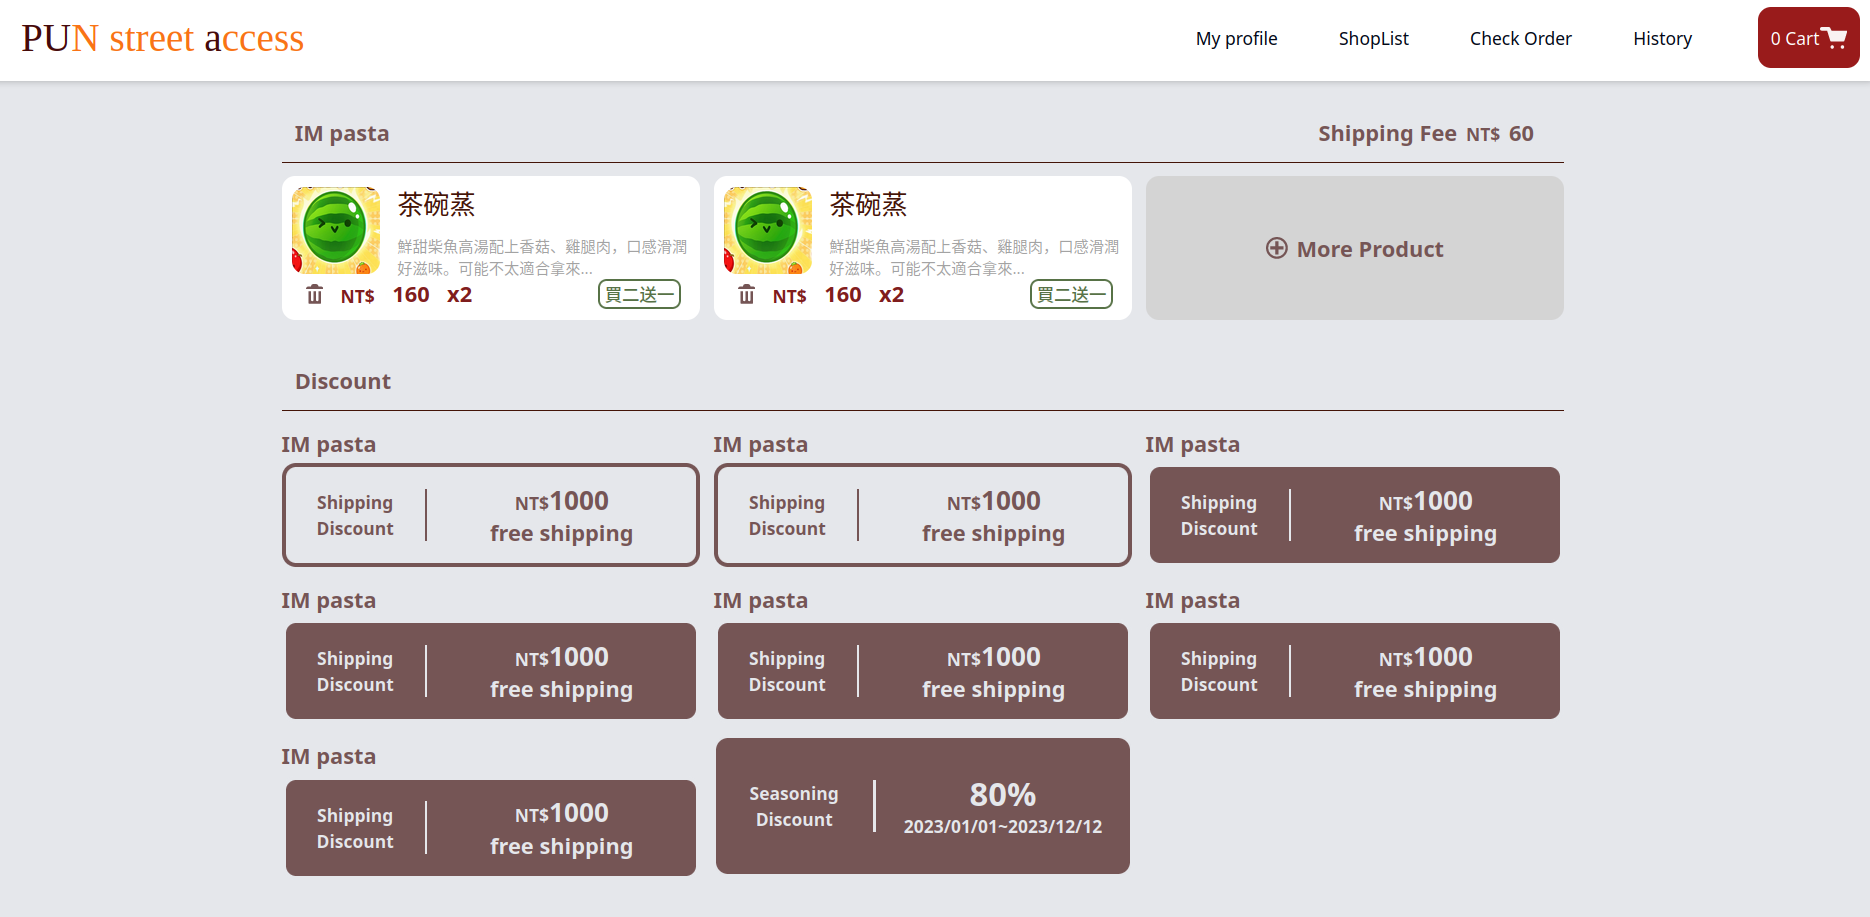
\includegraphics[width=40em]{pic/cart.png}}    
    \caption{cart page}
    \label{fig:enter-label}
\end{figure}

\newpage

\section{Glossary}
\newpage


\section{References}
\printbibliography[heading=none]
\newpage

\section{Appendix}
\newpage

\end{document}
